% Format teze zasnovan je na paketu memoir
% http://tug.ctan.org/macros/latex/contrib/memoir/memman.pdf ili
% http://texdoc.net/texmf-dist/doc/latex/memoir/memman.pdf
% 
% Prilikom zadavanja klase memoir, navedenim opcijama se podešava 
% veličina slova (12pt) i jednostrano štampanje (oneside).
% Ove parametre možete menjati samo ako pravite nezvanične verzije
% mastera za privatnu upotrebu (na primer, u b5 varijanti ima smisla 
% smanjiti 
\documentclass[12pt,oneside]{memoir}

% Paket koji definiše sve specifičnosti mastera Matematičkog fakulteta
\usepackage{matfmaster}
\usepackage{minted}
\usemintedstyle{perldoc}
\usepackage{listings}
\usepackage{url}
\renewcommand\listingscaption{Kод}
%
% Podrazumevano pismo je ćirilica.
%   Ako koristite pdflatex, a ne xetex, sav latinički tekst na srpskom jeziku
%   treba biti okružen sa \lat{...} ili \begin{latinica}...\end{latinica}.
%
% Opicija [latinica]:
%   ako želite da pišete latiniciom, dodajte opciju "latinica" tj.
%   prethodni paket uključite pomoću: \usepackage[latinica]{matfmaster}.
%   Ako koristite pdflatex, a ne xetex, sav ćirilički tekst treba biti
%   okružen sa \cir{...} ili \begin{cirilica}...\end{cirilica}.
%
% Opcija [biblatex]:
%   ako želite da koristite reference na više jezika i umesto paketa
%   bibtex da koristite BibLaTeX/Biber, dodajte opciju "biblatex" tj.
%   prethodni paket uključite pomoću: \usepackage[biblatex]{matfmaster}
%
% Opcija [b5paper]:
%   ako želite da napravite verziju teze u manjem (b5) formatu, navedite
%   opciju "b5paper", tj. prethodni paket uključite pomoću: 
%   \usepackage[b5paper]{matfmaster}. Tada ima smisla razmisliti o promeni
%   veličine slova (izmenom opcije 12pt na 11pt u \documentclass{memoir}).
%
% Naravno, opcije je moguće kombinovati.
% Npr. \usepackage[b5paper,biblatex]{matfmaster}

% Pomoćni paket koji generiše nasumičan tekst u kojem se javljaju sva slova
% azbuke (nema potrebe koristiti ovo u pravim disertacijama)
\usepackage{pangrami}

% Datoteka sa literaturom u BibTex tj. BibLaTeX/Biber formatu
\bib{matfmaster-primer}

% Ime kandidata na srpskom jeziku (u odabranom pismu)
\autor{Стефана Церовина}
% Naslov teze na srpskom jeziku (u odabranom pismu)
\naslov{Виртуелна машина Дартино- имплементација интерпретатора за платформу МИПС}
% Godina u kojoj je teza predana komisiji
\godina{2016}
% Ime i afilijacija mentora (u odabranom pismu)
\mentor{др Милена \textsc{Вујошевић Јаничић}\\ Универзитет у Београду, Математички факултет}
% Ime i afilijacija prvog člana komisije (u odabranom pismu)
\komisijaA{др Саша \textsc{Малков}\\ Универзитет у Београду, Математички факултет}
% Ime i afilijacija drugog člana komisije (u odabranom pismu)
\komisijaB{др Филип \textsc{Марић}\\ Универзитет у Београду, Математички факултет}
% Ime i afilijacija trećeg člana komisije (opciono)
% \komisijaC{}
% Ime i afilijacija četvrtog člana komisije (opciono)
% \komisijaD{}
% Datum odbrane (obrisati ili iskomentarisati narednu liniju ako datum odbrane nije poznat)
%\datumodbrane{}

% Apstrakt na srpskom jeziku (u odabranom pismu)
\apstr{%
Интернет и напредовање технологије омогућују уграђивање сензора и механизама комуникације у све већи број свакодневних предмета. Трансформацијом огромног броја предмета у паметне уређаје, и њиховим повезивањем кроз мрежу, гради се систем који се назива ИоТ. Овај термин указује на проширивање интернета у још већу мрежу која повезује све што нас окружује. Сматра се да ће ИоТ направити једну од највећих револуција у технологији, и да је прва фаза револуције почела. Физички свет полако постаје тип информационог система, а све то пружа могућности за развијање великог броја нових апликација, које обећавају побољшање квалитета наших живота.

Паметни уређаји представљају системе са уграђеним рачунаром, који се заснивају на микропроцесорима или микроконтролерима. Апликације за микроконтролере до сада су развијане углавном у асемблерском језику или Ц-у, због чега је процес развоја доста спорији од развоја мобилних или веб апликација. Дартино је пројекат компаније Гугл (енг.~\textit{Google}) који има за циљ да омогући употребу програмског језика Дарт за програмирање микроконтролера, и тиме развој апликација приближи и олакша што већем броју програмера. Дарт је објектно-оријентисани програмски језик, иницијално развијен за писање веб апликација, са синтаксом која је слична Ц-у, па је лак за употребу и не захтева много учења. Циљ овог рада је да се омогући коришћење Дартино виртуелне машине на микроконтролерима са МИПС процесором, имплементацијом интерпретатора за МИПС. Мотивација за то је чињеница да су МИПС процесори трећи по заступљености на тржишту система са уграђеним рачунаром.
}

% Ključne reči na srpskom jeziku (u odabranom pismu)
\kljucnereci{ИоТ, програмски језик Дарт, виртуелна машина Дартино, МИПС}

\begin{document}
% ==============================================================================
% Uvodni deo teze
\frontmatter
% ==============================================================================
% Naslovna strana
\naslovna
% Strana sa podacima o mentoru i članovima komisije
\komisija
% Strana sa posvetom (u odabranom pismu)
\posveta{Брату, мами и тати}
% Strana sa podacima o disertaciji na srpskom jeziku
\apstrakt
% Sadržaj teze
\tableofcontents*

% ==============================================================================
% Glavni deo teze
\mainmatter
% ==============================================================================

% ------------------------------------------------------------------------------
\chapter{Увод}
Појам ,,Интернет ствари'' (енг.~\textit{Internet of things}), скраћено ИоТ (енг.~\textit{IоТ}), се све чешће среће, и он представља модел повезаности објеката који чине систем у оквиру којег објекти међусобно комуницирају. Реч ,,ствар'' у оквиру појма ,,Интернет ствари'' се односи на систем са уграђеним рачунаром (енг.~\textit{embedded system}) који преноси и прима информације путем мреже \cite{iot}. Системи са уграђеним рачунаром су системи специјалне намене, који обављају једну или више функција које тој намени одговарају (паметни телефони, дигитални сатови, паметне утичнице, МП3 плејери, штампачи, дигиталне камере и друго). Модерни системи са уграђеним рачунаром су углавном базирани на микроконтролерима, а ређе на микропроцесорима, зато што микроконтролере карактерише ефикасно управљање процесима у реалном времену, масовна производња, ниска цена и мала потрошња електричне енергије \cite{embedded}. Сматра се да је потенцијал за развој индустрије система са уграђеним рачунаром велики, и да је будућност у изградњи велики ИоТ система.

Развијање апликација за системе са уграђеним рачунаром се обично своди на програмирање у асемблеру или у програмском језику Ц (енг.~\textit{C}). Најчешће се користе компилатори ГЦЦ (енг.~\textit{GCC}) или ЛЛВМ (енг.~\textit{LLVM}), а од алата за дебаговање, обично алат ГДБ (енг.~\textit{GDB}). Развојно окружење се најчешће налази на другом рачунару, јер микроконтролер садржи малу количину РАМ и флеш меморије, па се на  њему обично не може покренути ниједан регуларни оперативни систем, а и микролинукс често захтева више РАМ меморије од оне којом микроконтролер располаже. Због наведених услова, процес развоја апликација је доста захтеван, подложан грешкама па због тога и спор.

Пошто се веб апликације много брже развијају од апликација за системе са уграђеним рачунаром, компанија Гугл је дошла на идеју да омогући програмирање система са уграђеним рачунаром у вишем програмском језику Дарт, за који постоји подршка за развој веб, серверских и мобилних апликација. Више о програмском језику Дарт речено је у глави \ref{chp:dart}.

Дарт је прилагођен специфичностима микроконтролера кроз нову библиотеку ,,dartino''. Тако је настала виртуелна машина Дартино, са намером да се програмирање система са уграђеним рачунаром олакша и приближи што већем броју програмера. Дартино омогућава писање апликација за мале микроконтролере, на језику који доста личи на Ц, али је објектно-оријентисан и садржи разне погодности које процес имплементације доста олакшавају, те се апликације могу развијати брже и ефикасније. Ова виртуелна машина је детаљније описана у глави \ref{chp:dartino}.

У оквиру Дартино виртуелне машине постојала је подршка за миктроконтролере са Интел и Арм архитектуром процесора. Због широке распрострањености МИПС процесора у системима са уграђеним рачунаром, у оквиру овог рада развијен је интерпретатор за платформу МИПС који је и званично интегрисан у Дартино пројекат. Имплементација интерпретатора описана је у глави \ref{chp:implementacija}, док је платформа МИПС детаљније описана у глави \ref{chp:mips}.\\

% ------------------------------------------------------------------------------



% ------------------------------------------------------------------------------
\chapter{МИПС}
\label{chp:mips}
% ------------------------------------------------------------------------------
У овој глави описана је МИПС архитектура процесора. У поглављу \ref{ciscrisc} описане су ЦИСК (енг.~\textit{CISC - Complex Instruction Set Computing}) и РИСК (енг.~\textit{RISC - Reduced Instruction Set Computing}) архитектуре процесора, док је у поглављу \ref{mips} описана архитектура МИПС. У поглављу \ref{sec:pipeline} је описана проточна обрада на РИСК и МИПС процесорима, а у поглављу \ref{delay-slot} је описан појам слот закашњења при скоковима и гранањима.  У поглављу \ref{sec:registers} су описани МИПС регистри. Скуп инструкција је описан у поглављу \ref{instructions}, а начини адресирања су описани у поглављу \ref{adresiranje}. Структура програма у МИПС асемблерском језику описана је у поглављу \ref{struktura}, а један пример МИПС позивне конвенције дат је у поглављу \ref{konvencija}.


\section{ЦИСК и РИСК}
\label{ciscrisc}
Термин архитектура у рачунарству се користи да опише апстрактну машину која се програмира, а не стварну имплементацију те машине. Архитектура процесора у суштини дефинише скуп инструкција и регистара. Архитектура и скуп инструкција се једним именом називају ИСА (енг.~\textit{ISA - Instruction Set Architecture})\cite{isa}.

ЦИСК архитектуру процесора карактерише богат скуп инструкција. Главна идеја је смањивање броја инструкција по програму, при чему писање програма постаје ефикасније. Редуковањем броја инструкција по програму постиже се смањење времена извршавања. Инструкције могу бити различитих дужина, а сложеност се огледа у томе да једна инструкција може обављати више операција. На пример, инструкција може вршити учитавање вредности из меморије, затим примену неке аритметичке операције, и записивање резултата у меморији. Овако сложене инструкције захтевају комплексност процесорског хардвера и резултујуће архитектуре. То има за последицу и теже разумевање и програмирање таквих чипова, а поред тога и већу цену.
ЦИСК процесори се углавном користе на личним рачунарима, радним станицама и серверима, а пример таквог процесора је Интел x86 \cite{mips, risc_vs_cisc}.

РИСК архитектура процесора се заснива на поједностављеном и смањеном скупу инструкција. Због једноставности инструкција, потребан је мањи број транзистора за производњу процесора, при чему процесор инструкције може брже извршавати. Међутим, редуковање скупа инструкција умањује ефикасност писања софтвера за ове процесоре. 
Постоје 4 начина адресирања: регистарско, PC-релативно, псеудо-директно и базно. Не постоје сложене инструкције које приступају меморији, већ се рад са меморијом своди на \textit{load} и \textit{store} инструкције \cite{mips, risc_vs_cisc}. Више о начинима адресирања речено је у поглављу \ref{adresiranje}.
Највећа предност је проточна обрада, која се лако може имплементирати, за разлику од ЦИСК процесора код којих то није могуће. Више о проточној обради речено је у поглављу \ref{sec:pipeline}. РИСК процесори се углавном користе за апликације у реалном времену. Пример РИСК процесора су АРМ и МИПС .

\section{МИПС}
\label{mips}
МИПС је РИСК архитектура процесора, настала средином осамдесетих, као рад Џона Хенесија и његових студената на универзитету Станфорд. Истражујући РИСК, показали су да се помоћу једноставног скупа инструкција, добрих компилатора и хардвера који ефикасније користи проточну обраду, могу произвести бржи процесори на мањем чипу \cite{mips}.

Временом, МИПС архитектура је еволуирала на много начина. Направљена је подршка за 64-битно адресирање и операције, комплексне оперативне системе као што је Unix, као и високе перформансе при раду са бројевима у покретном зарезу. Употреба ових процесора је кроз време, у зависности од перформанси, била разнолика: радне станице, серверски системи, Сони и Нинтендо играчке конзоле, Циско рутери, ТВ сет-топ боксови, ласерски штампачи и друго \cite{mips}.
Приступачна цена интегрисаних кола заснованих на овој архитектури, ниска потрошња енергије и доступност алата за развој програмске подршке чине је погодном како за системе са уграђеним рачунаром, тако и за потрошачку електронику, играчке конзоле и друго.


\section{Проточни систем }
\label{sec:pipeline}
Проточна обрада (енг. ~\textit{pipeline}) настала је из чињенице да различите фазе у току извршавања инструкције користе различите ресурсе. Уколико би трајање фаза било једнако, могао би се направити систем у ком по завршетку једне фазе текуће инструкције, почиње та фаза наредне инструкције. Овакав начин обраде инструкција назван је проточна обрада \cite{mips}. Да би се омогућило једнако трајање фаза, РИСК дефинише скуп инструкција у коме је количина посла која се извршава у оквиру једне инструкције максимално смањена. Да би се постигла једнакост трајања фазе декодирања инструкције, већина РИСК архитектура, међу којима је и МИПС, има фиксирану величину инструкција \cite{mips}.

Предуслов за ефикасну проточну обраду је коришћење кеш меморије ради убрзања приступа меморији. Кеш меморија је мала, брза, локална меморија која служи за складиштење копија меморијских података \cite{mips}. Сваки податак у кешу има показивач на адресу у главној меморији, на којој се налази. У кешу се чувају подаци које је процесор читао из меморије у најскорије време. Уколико је кеш пун, пребришу се најстарији подаци. При читању, прво се проверава да ли се податак налази у кешу. Уколико се не налази, долази до “промашаја кеша”. Промашај кеша се дешава ретко, отприлике у 10\% случајева.

У РИСК архитектури кеш је део процесора и везан је за проточну обраду, док је код ЦИСК архитектуре кеш меморија део меморијског система. МИПС има одвојен инструкцијски кеш и кеш података, тако да се у исто време може читати инструкција из меморије и читати или уписивати подаци. 

\subsection{Проточна обрада на МИПС платформи}

Извршавање сваке инструкције је подељено у 5 фаза, при чему свака фаза има фиксирано трајање. Прва, трећа и четврта фаза трају по један радни такт процесора , док друга и пета трају по пола такта, тако да укупно извршавање инструкције траје 4 такта \cite{mips}. У наставку ће бити описана свака од фаза.

\begin{enumerate}
\item Дохватање инструкције из инструкцијског кеша - декодирање инструкције (енг.~instruction fetch, скраћено IF)
\item Читање садржаја одговарајућих регистара (операнада инструкције) (енг.~read register, скраћено RR)
\item Извршавање аритметичко/логичких операција у једном радном такту (операције у покретном зарезу, множење и дељење се раде другачије) (енг.~arithmetic/logic unit, скраћено ALU)
\item  Фаза у којој се дохватају/пишу подаци у меморију. Углавном 3 од 4 инструкције не раде ништа у овој фази, али постоји да не би дошло до тога да две инструкције у исто време желе да приступе кешу (енг.~memory, скраћено MEM)
\item Вредност(резултат) операције се уписује у регистар (енг.~write back, скраћено WB)
\end{enumerate}

На слици \ref{fig:pipeline} је приказано извршавање 3 инструкције на платформи МИПС. Када се заврши прва фаза прве инструкције, из меморије се дохвата друга инструкција. Са завршетком прве фазе друге инструкције, почиње прва фаза треће инструкције итд. 

\begin{figure}[!ht]
  \centering
  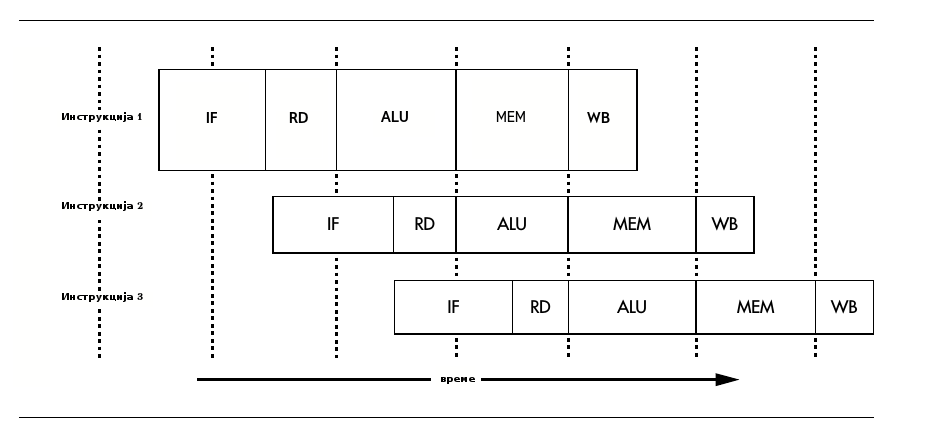
\includegraphics[width=0.9\textwidth]{pipeline.png}
  \caption{Проточна обрада на платформи МИПС.}
  \label{fig:pipeline}
\end{figure}

Ефикасна проточна обрада има за последицу следеће \cite{mips}:
\begin{enumerate}
\item Све инструкције морају бити исте дужине, што ограничава комплексност инструкција. На платформи МИПС је та дужина 32 бита. Више о МИПС инструкцијама речено је у поглављу \ref{instructions}
\item Подацима се приступа само у фази 4
\item Приступ меморији омогућен само помоћу инструкција \textit{load} и \textit{store}
\item Аритметичко/логичке инструкције имају три операнда
\item Нема специјалних инструкција чија комплексност лоше утиче на ефикасност проточне обраде
\item Постоје 32 регистра опште намене чија  величина зависи од тога да ли је архитектура 32-битна или 64-битна. Више о MИПС регистрима речено је у поглављу \ref{sec:registers}
\end{enumerate}

\section{Слот закашњења}
\label{delay-slot}

Структура проточног система МИПС процесора је таква да када инструкција скока или гранања дође у фазу извршавања, инструкција након скока/гранања ће већ бити започета. Пошто ово може бити предност, дефинисано је да се инструкција која следи након скока/гранања мора извршити пре скока. Позиција инструкције која следи након скока/гранања назива се слот закашњења гранања (енг.~\textit{Branch delay slot}). Када је то могуће, углавном се у слот закашњења смешта инструкција која  би иначе била пре скока/гранања. То се не може применити када је у питању условни скок. У случајевима када се ништа не може ставити у слот закашњења, попуњава се инструкцијом \textit{nop} \cite{mips}.

Још једна последица проточне обраде је што подаци дохваћени \textit{load} инструкцијом стижу тек након инструкције која се налази иза \textit{load}. Последица је да се ти подаци не могу користити одмах у наредној инструкцији. Позиција инструкције која следи одмах иза \textit{load} се назива слот закашњења учитавања (енг.~\textit{Load delay slot}). На модерним процесорима резултат \textit{load} инструкције је блокиран. Ако се покуша са приступом резултату, зауставља се извршавање и чека се да подаци стигну \cite{mips}. 

\section{Регистри}
\label{sec:registers}
Регистри представљају малу, веома брзу меморију, која је део процесора. МИПС процесори могу вршити операције само над садржајима регистара и специјалним константама које су део инструкције.

У МИПС архитектури, постоје 32 регистра опште намене \cite{mips}: \textit{\$0} - \textit{\$31}. Два регистра имају другачије понашање од осталих: 
\begin{itemize}
\item \textbf{\$0} Увек враћа 0, без обзира на садржај.
\item \textbf{\$31} Увек се користи за адресу повратка из функције на коју се скочи инструкцијом \textit{jal}.
\end{itemize}

Постоје два специјална регистра \textit{Hi} и \textit{Lo}, који се користе само при множењу и дељењу. Ово нису регистри опште намене, те се не користе при другим инструкцијама. Не може им се приступити директно, већ постоје специјалне инструкције \textit{mfhi} и \textit{mflo} за премештање садржаја ових регистара \cite{mips}.

У наставку ће бити описани регистри опште намене \cite{mips}:

\begin{itemize}
\item \textbf{at} - Резервисан је за псеудоинструкције генерисане од стране асемблера. Псеудоинструкције нису праве инструкције, већ су уведене како би се се олакшало програмирање у МИПС асемблерском језику. Њих асемблер преводи у две или више правих инструкција из скупа инструкција.

\item \textbf{v0, v1} - Користе се за враћање резултата при повратку из неке функције. Резултат може бити целобројног типа или број записан у фиксном зарезу.

\item \textbf{a0 - a3} - Користе се за прослеђивање прва 4 аргумента функцији која се позива. 

\item \textbf{t0 - t9} - По конвенцији која је описана у поглављу \ref{konvencija}, функције могу користи ове регистре без потребе да њихов садржај сачувају пре тога. Зато се могу користити као “променљиве” при израчунавањима, само се мора водити рачуна да ће се при позиву неке друге функције садржај тих регистара изгубити.

\item \textbf{s0 - s7} - По конвенцији која је описана у поглављу \ref{konvencija}, функција мора обезбедити да ће садржај ових регистара при уласку у функцију бити исти као и при изласку из ње. То се обезбеђује или некоришћењем, или чувањем садржаја на стеку на почетку функције, пре коришћења, и скидањем садржаја са стека пре изласка из функције.

\item \textbf{k0, k1} - Резервисано за систем прекида, који након коришћења не враћа садржај на почетни.

\item \textbf{gp} - Користи се у различите сврхе. У коду који не зависи од позиције (енг.~\textit{Program Independent Code}, скраћено \textit{PIC}), свом коду и подацима се приступа преко табеле показивача, познате као ГОТ (енг.~\textit{Global Offset Table}). Регистар \textit{\$gp} показује на ту табелу.
У регуларном коду који зависи од позиције, може се користи као показивач на средину у статичкој меморији. То значи да се подацима који се налазе 32 бита лево и десно од овог регистра може приступити помоћу једне инструкције, тако што се овај регистар користи као базни. У пракси се на ове локације смештају глобални подаци који не заузимају много меморије.

\item \textbf{sp} - Показивач на стек. Потребне су специјалне инструкције да би се показивач на стек повећао и смањио, тако да МИПС ажурира стек само при позиву и повратку из функције. Одговорност је на функцији која је позвана. \textit{\$sp} се при уласку у функцију прилагођава на најнижу тачку на стеку којојој ће се приступати у функцији. Тако је омогућено да компилатор може да приступи променљивама на стеку помоћу константног помераја у односу на \textit{\$sp}.

\item \textbf{fp} - Познат и као \textit{\$s8} , показивач на стек оквир. Користи се од стране функције, за праћење стања на стеку, за случај да из неког разлога компилатор или програмер не могу да израчунају померај у односу на \textit{\$sp}. То се може догодити уколико пограм врши проширење стека, при чему се вредност проширења рачуна у току извршавања. Ако се дно стека не може израчунати у току превођења, не може се приступити променљивама помоћу \textit{\$sp}, па се на почетку функције \textit{\$fp} иницијализује на константну позицију која одговара стек оквиру функције. Ово је локално за функцију.

\item \textbf{ra} - При уласку у функцију овај регистар обично садржи адресу повратка функције, тако да се функције углавном завршавају инструкцијом \textit{jr \$ra}. У принципу, може се користити било који регистар, али неке оптимизације које врши процесор ће радити боље уколико се користи ra (нпр.~предвиђање гранања (енг.~\textit{branch prediction})). Функције које позивају друге функције морају сачувати садржај регистра \textit{\$ra}.
\end{itemize}

Постоје два формата за адресирање: коришћењем бројева \textit{\$0-\$31} или коришћењем имена \textit{\$а0, \$s0, \$t0} и слично.

\section{Скуп инструкција}
\label{instructions}
У МИПС асемблерском језику постоје следеће инструкције \cite{mips1}:
\begin{itemize}
\item аритметичке: сабирање, одузимање, множење, дељење
\item логичке: и, или, шифтовање у лево, шифтовање у десно
\item приступ меморији: учитавање речи, записивање речи у меморију
\item гранање
\item скокови
\end{itemize}
На основу типова операнада, све МИПС инструкције се могу поделити у три типа \cite{mips}

\textbf{Р} - Инструкције које као операнде очекују регистре.
Представљају се следећим форматом:
\begin{listing}
\centering
\textbf{OP rd, rs, rt}
\end{listing}

\textit{OP} представља ознаку одређене инструкције, \textit{rd} представља регистар за смештање резултата, док \textit{rs, rt} означавају операнде.

Неке од инструкција које припадају Р типу:

\begin{itemize}
\item jr - Скакање на адресу у регистру
\item slt - Постави 1 у регистар за резултат уколико је вредност у првом регистру мања од вредности у другом
\item srl - Логичко шифтовање у десно
\end{itemize}

\textbf{И} - Инструкције које имају као операнде регистар и константну вредност се представљају следећим форматом:
\begin{listing}
\centering
\textbf{OP rd, rs, Imm}
\end{listing}

\textit{OP} представља ознаку одређене инструкције, \textit{rd} представља регистар за смештање резултата, \textit{rs} представља први операнд који је регистар, док је \textit{Imm} константа која је други операнд. Константа може имати највише 16 бита.

Неке од инструкција које припадају И типу:

\begin{itemize}
\item addi - Сабирање вредности у регистру и константе
\item slti - Постави 1 у регистар за резултат уколико је вредност у првом регистру мањи од константе
\item beq - Гранање у случају да је вредност у првом регистру једнака константи
\end{itemize}

\textbf{J} - Инструкције које се користе при скоковима.
Представљају се следећим форматом:
\begin{listing}
\centering
\textbf{ј label}
\end{listing}

Постоје две ,,ј'' инструкције: \textit{j} и \textit{jal}. Инструкцијом \textit{j - Jump }процесор се пребаца на извршавање инструкције која се налази на адреси \textit{label}. Инструкција \textit{jal - Jump and link} ради исто то, али смешта адресу наредне инструкције у регистар \textit{\$ra}, тако да се након завршетка функције на коју се скочило, може наставити са извршавањем. Ове инструкције имају највише места за константу- 26 бита, јер су адресе велики бројеви.

\section{Начини адресирања}
\label{adresiranje}

На платформи МИПС постоје четири начина адресирања \cite{mips}:

\begin{description}
\item Регистарско

Регистарско адресирање се користи у \textit{jr} инструкцији. Пошто је величина регистра 32 бита, а било која адреса је такође 32 бита, на овај начин се може приступити било којој адреси. У наставку је дат пример инструкције са регистарским адресирањем.
\begin{listing}
\centering
\textbf jr rs
\end{listing}

\item PC-релативно

PC-релативно адресирање се користи у \textit{beq}, \textit{bne} и другим инструкцијама гранања. Ово су инструкције И типа. Константа која представља адресу може имати највише 16 бита, што значи да се не може приступити великом броју адреса. Ове инструкције се углавном користе за скокове на инструкције које су близу, а адреса се рачуна као PC + константа. У наставку је дат пример инструкције са PC-релативним адресирањем.
\begin{listing}
\centering
\textbf bne rs, rt, imm
\end{listing}

\item Псеудо-директно

Директно адресирање би значило да се у инструкцији наводи адреса. То је немогуће зато што адреса има 32-бита, колико и цела инструкција. Псеудо-директно адресирање се користи у инструкцији \textit{j}. За операцију се користи 6 бита, тако да за адресу остаје 26. Адресирање се изводи тако што се горња 4 бита позајме од PC-a, а на крај се дода 00. У наставку је дат пример инструкције са псеудо-директним адресирањем.

\begin{listing}
\centering
\textbf j imm
\end{listing}

\item Базно

Базно адресирање подразумева рачунање адресе као збира садржаја регистра и помераја. Овај тип адресирања примељује се код инструкција \textit{lw} и \textit{sw}. Константа која представља померај може имати највише 16 бита.

\begin{listing}
lw rt, offset(rs)
\centering
\end{listing}
\end{description}

\section{Структура програма}
\label{struktura}
У Фон Нојмановим архитектурама, међу којима је и МИПС, подаци и к\^{о}д се налазе у истој меморији. То захтева да се меморија подели на два сегмента, сегмент података и кодни сегмент.

У сегменту података налазе се декларације имена променљивих које се користе у програму, чиме се за сваку променљиву алоцира меморија. Означава се асемблерском директивом \textbf{.data}. Декларација се састоји из имена променљиве, након чега следи ,,:'' тип и вредност \cite{mips}.

Кодни сегмент се означава директивом \textbf{.text} и састоји се из инструкција. Почетна тачка за извршавање програма означава се лабелом \textbf{main:}, а крај \textit{main} дела се означава позивом \textit{syscall}. Овим позивом, контрола се преноси оперативном систему, који на основу садржаја регистра \textit{\$v0} зна шта треба да уради \cite{mips}.

\begin{listing}
\begin{minted}[bgcolor=olive!10]{text}
  .data
 hello:     .asciiz "Zdravo svete!"
 length:    .word   12
            .globl main
  .text

 main:
    li  a0, 1
    la  a1, hello
    lw  a2, length
    li  v0, 15
    syscall
end:
    li        v0, 10
    syscall
\end{minted}
\caption{Програм који исписује поздравну поруку, у МИПС асемблерском језику.}
\label{asmkod}
\end{listing}

Кодом \ref{asmkod} је приказан пример програма у МИПС асемблерском језику. Овај програм исписује поздравну поруку на стандарадни излаз, на следећи начин:
\begin{enumerate}
\item Најпре се директивом \textit{.data} означи да након те линије почиње декларација променљивих.
\item Затим се декларише ниска \textit{,,hello''}, која је типа \textit{asciiz} (ниске овог типа се завршавају \textit{NULL} карактером, и фиксиране су дужине). Вредност ниске се постави на \textit{,,Zdravo svete!''}.
\item Након тога се декларише променљива која представља дужину ниске \textit{,,hello''}.
\item Директива \textit{.globl} означава да је симбол \textit{main} доступан ван ове асемблерске датотеке.
\item Након тога се означи почетак кодног сегмента директивом \textit{.text}.
\item Лабела \textit{main} означава почетак прве инструкције која се извршава.
\item У регистар \textit{\$a0} учита се први аргумент системског позива \textit{write} - 1 oзначава да се резултат исписује на стандардни излаз.
\item У регистар \textit{\$a1} учита се други аргумент, ниска која се исписује.
\item У регистар \textit{\$a2} учита се трећи аргумент који представља дужину ниске.
\item У регистар \textit{\$v0} учита се к\^{о}д за системски позив \textit{write}.
\item Након тога се контрола прослеђује оперативном систему који исписује ниску.
\item Лабела \textit{ end:} означава крај програма.
\item У регистар \textit{\$v0} учита се к\^{о}д за системски позив \textit{exit}.
\item Након тога се позива оперативни систем да прекине извршавање програма.
\end{enumerate}


\section{Позивна конвенциja}
\label{konvencija}

Позивна конвенција представља правила рада са регистрима и стек оквиром приликом позива функције. Не постоји јединствена МИПС позивна конвенција која се мора примењивати, тако да ће овде бити представљена она која је коришћена при имплементацији МИПС интерпретатора у оквиру Дартино виртуелне машине.

При позиву неке функције, на стеку се прави посебан стек оквир, и то се дешава за сваки позив, односно за сваку инстанцу једне функције. Организација стек оквира дефинише однос између позиваоца и позване функције, који се односи на начин прослеђивања аргумената и резултата, и дељења регистара. Поред тога, дефинише и организацију локалног складишта позване функције унутар њеног стек оквира \cite{konvencija}.

\begin{figure}[!ht]
  \centering
  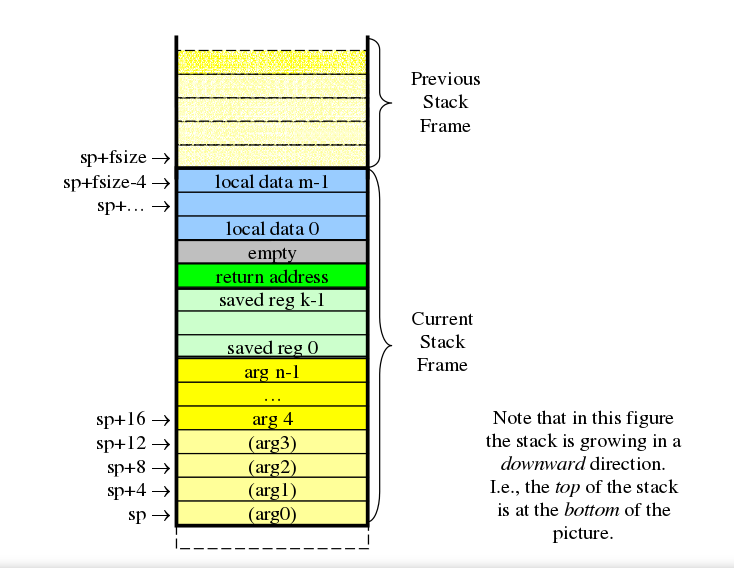
\includegraphics[width=0.8\textwidth]{stack_frame.png}
  \caption{Организација стек оквира.}
  \label{fig:stack_frame}
\end{figure}

Стек оквир функције се дели на 5 региона, што је приказано на слици \ref{fig:stack_frame}. У наставку ће бити описан сваки од њих \cite{konvencija}.

\begin{enumerate}

\item Први регион представља простор за смештање аргумената, који се прослеђују функцијама које се позивају из тренутне функције (тренутна функција је она чији се стек оквир налази на врху стека). Прва четири места никад не користи тренутна функција, већ функција која је позвана. Уколико је потребно проследити више од 4 аргумента, они се смештају на адресе \textit{\$sp+16},\textit{\$sp+20}, \textit{\$sp+24} итд.

\item Други регион представња простор за смештање садржаја регистара чувања (\textit{\$s0-\$s7}) које тренутна функција жели да користи. При уласку у функцију, садржаји регистара које ће функција користити се сачувају на стеку, а пре изласка се врате на оригиналне. Циљ је да функција која је позвала тренутну функцију има исте садржаје ових регистара пре и после позива.

\item У трећем региону се смешта адресе повратка функције, односно садржај регистра \textit{\$ra}. Ова вредност се копира на стек при уласку у функцију, и копира назад у регистар  \textit{\$ra} пре изласка из функције.

\item Четврти регион представља поравнање стек оквира на адресу која је дељива са 8. То је овде неопходно да би секција локалних података почела на адреси која је дељива са 8.

\item Пети регион је секција за складиштење локалних података. Функција овде мора резервисати место за све локалне променљиве, као и за све привремене регистре (\textit{\$t0-\$t9}), које мора сачувати пре позивања друге функције. Ова секција такође мора бити поравната на 8.
\end{enumerate}

Позивна конценција уводи и нека додатна правила:
\begin{itemize}

\item Вредност показивача на стек увек мора бити дељива са 8. Ово обезбеђује да се 64-битни подаци увек могу сместити на стек без генерисања грешке поравнања адреса у току извршавања. Из овога следи да величина сваког стек оквира мора бити дељива са 8.

\item Вредности регистара аргумената се не морају чувати при позиву функције. Функција може мењати ове регистре, без чувања њихове претходне вредности.

\item Прва 4 места у секцији аргумената су позната као слотови аргумената - меморијске локације које су резервисане за смештање 4 аргумента \textit{\$а0-\$а3}. Функција не чува ништа на овим позицијама, јер се аргументи прослеђују кроз регистре \textit{\$а0-\$3}. Међутим, позвана функција може у слотовима аргумената сачувати вредности ових регистара, уколико то жели.

\item Свака функција мора у оквиру свог стек оквира алоцирати меморију за максималан број аргумената за било коју функцију коју позива. Уколико функција коју позива има мање од 4 аргумента, онда мора резервисати 4.
\end{itemize}


% ------------------------------------------------------------------------------
\chapter{Програмски језик Дарт}
\label{chp:dart}
% ------------------------------------------------------------------------------
У овој глави описане су карактеристике програмског језика Дарт. У поглављу \ref{tipovi} описано је на који начин су подржани типови, док су у поглављу \ref{klase} описане специфичности при раду са класама. Рад са библиотекама је описан у поглављу \ref{dart_biblioteke}. Подршка за асинхроност описана је у поглављу \ref{asinhronost}, а подршка за конкуретне процесе описана је у поглављу \ref{dart_izolate}. У поглављу \ref{funkcije} описан је рад са функцијама, док је у поглављу \ref{metapodaci} описан појам метаподатака. Разлике Дарта у односу на Јаваскрипт описане су у поглављу \ref{specificnosti}.

\section{Основне карактеристике}
Дарт је објектно-оријентисани језик, који се заснива на класама и једноструком наслеђивању. Дарт се обично користи код програмирања веб апликација, али се може користити и за мобилне апликације, веб сервере, и програмирање система са уграђеним рачунаром.

Дарт је уско везан за Јаваскрипт. Програми написани у Дарту се могу превести у Јаваскрипт. При покретању у веб прегледачу, преводи се у Јаваскрипт помоћу \textit{dart2js} компилатора, при чему се врши оптимизација Јаваскрипт кода. У неким случајевима, к\^{о}д написан у Дарту се брже извршава од одговарајућег кода написаног у Јаваскрипту \cite{dart, dart1}.

У наставку су описани неки од најважнијих концепата програмског језика Дарт \cite{dart, dart1}.
\begin{itemize}
\item Свака променљива је објекат, при чему сви објекти наслеђују класу Object.
\item Навођење типова је опционо, али постоји подршка и за статичку проверу типова.
\item Могу се креирати анонимне функције и затворења.
\item Нема кључних речи \textit{public}, \textit{private} и \textit{protected}. Идентификатори који почињу доњом цртом су приватни.
\item Постоји подршка за асинхроно програмирање и за конкурентно извршавање.
\item Метаподаци се користе за пружање додатних информација о коду.
\end{itemize}

\section{Типови}
\label{tipovi}

У Дарту се типови не морају наводити, али је препоручљиво. У званичном упутству стоји да би требало наводити типове у класама и методама. Тиме се смањује количина грешака, при чему не постоји провера типова у току извршавања, већ само у току превођења. Навођењем типова к\^{о}д је уједно лакши за читање и пружа бољу документацију \cite{dart, dart1}. 

\section{Класе}
\label{klase}
Као објектно-оријентисани језик, Дарт је заснован на класама и једноструком наслеђивању. Иако свака класа може имати само једну надкласу, могуће је имплементирање више интерфејса, при чему свака класа може бити интерфејс за неку другу класу. 

Класа може садржати тело друге класе (енг.~\textit{Mixins}). К\^{о}д неке друге класе се може искористити помоћу кључне речи ~\textit{with} након које следи име класе чији се к\^{о}д копира (\textit{Mixin}). Кодом \ref{usemixin} представљена је класа која користи уметнуте класе \textit{Musical} и \textit{Aggressive} \cite{dart, dart1}.

\begin{listing}
\begin{minted}[bgcolor=olive!10]{javascript}
class Maestro extends Person
    with Musical, Aggressive{
  Maestro(String maestroName) {
    name = maestroName;
    canConduct = true;
  }
}
\end{minted}
\caption{Пример класе која користи \textit{Mixin}.}
\label{usemixin}
\end{listing}

Да би се класа могла уметнути она се креира као класа која нема конструктор. Кодом \ref{mixin} представљена је класа која се може уметнути.

\begin{listing}
\begin{minted}[bgcolor=olive!10]{javascript}
abstract class Musical {
  bool canPlayPiano = false;
  bool canCompose = false;
  bool canConduct = false;

  void entertainMe() {
    if (canPlayPiano) {
      print('Playing piano');
    } else if (canConduct) {
      print('Waving hands');
    } else {
      print('Humming to self');
    }
  }
}
\end{minted}
\caption{Пример \textit{Mixin} класе.}
\label{mixin}
\end{listing}

Још једна важна карактеристика Дарта је да се конструктори не наслеђују. Уколико класа нема дефинисан конструктор, Дарт ће јој доделити подразумевани. Не може се дефинисати више конструктора, али се могу креирати именовани конструктори. Kодом \ref{named_constructor} представљено је дефинисање именованог конструктора \cite{dart, dart1}:
\begin{listing}
\begin{minted}[bgcolor=olive!10]{javascript}
class Point {
  num x;
  num y;

  Point(this.x, this.y);

  Point.fromJson(Map json) {
    x = json['x'];
    y = json['y'];
  }
}
\end{minted}
\caption{Пример дефинисања именованог конструктора.}
\label{named_constructor}
\end{listing}
\section{Библиотеке}
\label{dart_biblioteke}
Свака Дарт апликација је библиотека, чак и ако нема кључну реч \textit{library}. Кључна реч \textit{import} користи се за укључивање одређене библиотеке, при чему постоји могућност лењог учитавања библиотеке помоћу \textit{deferred as}. Лењо учитавање може смањити време покретања апликације, а користи се и када постоје функционалности које се ретко користе. Пример лењог учитавања дат је кодом \ref{lazy1}. Када нам је потребна лењо учитана библиотека, укључујемо је функцијом \textit{loadLibrary()}, што је представљено кодом \ref{lazy2} \cite{dart, dart1}.

\begin{listing}
\begin{minted}[bgcolor=olive!10]{javascript}
import 'package:deferred/hello.dart' deferred as hello;
\end{minted}
\caption{Пример лењог учитавања класе.}
\label{lazy1}
\end{listing}

\begin{listing}
\begin{minted}[bgcolor=olive!10]{javascript}
greet() async {
  await hello.loadLibrary();
  hello.printGreeting();
}
\end{minted}
\caption{Пример укључивања лењо учитане библиотеке.}
\label{lazy2}
\end{listing}

\section{Функције}
\label{funkcije}
Пошто је Дарт чисто објектно-оријентисани језик, и функције су објекти, типа \textit{Function}. То значи да се функције могу додељивати променљивама, или прослеђивати као аргументи функције \cite{dart, dart1}.

Функције које садрже само један израз, могу се записивати у скраћеном облику, што је представљено кодом \ref{arrowfunc}. 
\begin{listing}
\begin{minted}[bgcolor=olive!10]{javascript}
bool funkcija(int arg) => izraz;
\end{minted}
\caption{Пример скраћеног облика записивања функција.}
\label{arrowfunc}
\end{listing}

Такође, у Дарту постоје анонимне функције које се могу креирати на начин приказан кодом \ref{anfunction}. Променљивој \textit{func} додељује се анонимна функција која штампа поруку великим словима \cite{dart, dart1}.

\begin{listing}
\begin{minted}[bgcolor=olive!10]{javascript}
var func = (msg) => print(msg.toUpperCase());
func('Hello');
\end{minted}
\caption{Пример коришћења анонимне функције која штампа елемент листе.}
\label{anfunction}
\end{listing}

Могу се креирати затворења, која представљају функције која памте контекст у ком су креиране (могу приступати променљивама које су дефинисане у контексту у ком су креиране). Пример затворења дат је кодом \ref{closure}. Функција \textit{makeAdder} враћа као резултат функцију која додаје број \textit{addBy} аргументу те функције, односно враћа затворење.  Ово затворење ће имати приступ променљивој за коју је креирано. На почетку је променљива \textit{pom} иницијализована на 3. Након тога се креира објекат функције \textit{makeAdder}, са аргументом \textit{pom}, који се додели променљивој \textit{add}. При позиву ове функције са аргументом 5, резултат ће бити 8. Након што променимо вредност променљиве \textit{pom} на 7, позив функције за аргумент 5 ће вратити 12, јер се унутар затворења приступа тренутној вредности променљиве \cite{dart, dart1}.

\begin{listing}
\begin{minted}[bgcolor=olive!10]{javascript}
Function makeAdder(num addBy) {
  return (num i) => addBy + i;
}

main() {
  var pom = 3;
  var add  = makeAdder(pom);
  add(5); // 8
  pom = 7;
  add(5); // 12
}
\end{minted}
\caption{Пример функције која враћа затворење.}
\label{closure}
\end{listing}

\section{Асинхроност}
\label{asinhronost}
Дарт има више начина за подршку асинхроног програмирања, а најчешће употребљивани су \textit{async} функције и \textit{await} изрази. Функције које враћају \textit{Future} или \textit{Stream} објекат су асинхроне. Асинхроне функције враћају као резултат операцију која ће се извршити у будућности.

\textit{Future} представља средство за враћање вредности некад у будућности. Када се позове функција која враћа \textit{Future}, та функција стане са извршавањем и врати непотпуни \textit{Future} објекат. Касније, када вредност коју треба да врати буде доступна, \textit{Future} објекат се допуни том вредношћу или врати грешку. Вредност коју представља \textit{Future} може се добити помоћу \textit{async} и \textit{await}, или помоћу \textit{Future} АПИ-ја \cite{dart, dart1}. 

Да би се користио \textit{await}, к\^{о}д мора бити унутар функције која је означена као \textit{async}. Пример у коме се помоћу \textit{await} чека на резултат асинхроне функције, дат је кодом \ref{async}. Функција \textit{lookUpVersion}, је нека асинхрона функција која враћа \textit{Future} \cite{dart, dart1}.

\begin{listing}
\begin{minted}[bgcolor=olive!10]{javascript}
checkVersion() async {
  var version = await lookUpVersion();
  if (version == expectedVersion) {
    // Do something.
  } else {
    // Do something else.
  }
}
\end{minted}
\caption{Пример употребе \texttt{await}.}
\label{async}
\end{listing}

\textit{Future} АПИ се користио док није додата подршка за \textit{async} и \textit{await}, а данас се углавном користи када су нам потребне функционалности које \textit{async} и \textit{await} не могу пружити.

\textit{Stream} представља секвенцу асинхроних догађаја, која може садржати догађаје генерисане од стране корисника, или податке прочитане из датотека.  Вредности из \textit{Stream}-а могу се добити помоћу \textit{await-for} или \textit{listen} из \textit{Stream} AПИ-ја. Пример асинхроне \textit{for} петље којом се итерира кроз догађаје стрима дат је кодом \ref{stream}. Како је овде стрим низ целобројних догађаја, у петљи се прихвата догађај стрима и додаје на суму. Када се петља заврши, функција се паузира док не стигне следећи догађај. Функција која користи \textit{await for} петљу мора се означити са \textit{async} \cite{dart, dart1}.

\begin{listing}
\begin{minted}[bgcolor=olive!10]{javascript}
Future<int> sumStream(Stream<int> stream) async {
  var sum = 0;
  await for (var value in stream) {
    sum += value;
  }
  return sum;
}
\end{minted}
\caption{Пример употребе прихватања догађаја \texttt{Stream}-а.}
\label{stream}
\end{listing}
\section{Изолате}
\label{dart_izolate}
Дарт програм се увек извршава у једној нити. Нема конкурентног извршавања са дељењем меморије, већ је конкурентност подржана кроз изолате (енг.~\textit{Isolates}).

Изолата је јединица конкурентног извршавања. Између изолата нема дељења меморије, а комуникација се обавља слањем порука кроз портове \textit{ReceivePort} и \textit{SendPort}. Свака изолата има своју хип меморију. Сваки Дарт програм се састоји из бар једне изолате, која се назива главна изолата (енг.~\textit{main isolate}) \cite{dart, dart1}. При превођењу на Јаваскрипт, изолате се преводе у веб воркере (енг.~\textit{Web Worker} \footnote{Појам који означава нешто између процеса и нити. Извршава се у позадини и тиме не утиче на одзивност система.}).

Пример комуникације изолата дат је кодом \ref{izolate_primer}. Функција \textit{Isolate.spawn} покреће нову изолату \textit{echo}. Овој изолати се прослеђује порт на ком изолата која ју је креирала (главна изолата) чека одговор. У оквиру ње се отвара порт на ком се примају одговори, а затим се тај порт шаље главној изолати. Након тога се у \textit{for} петљи помоћу \textit{await} чека да стигну подаци. Када податак стигне, шаље се на \textit{SendPort}. У \textit{main} функцији се након креирања изолате, прима порт који је \textit{echo} изолата послала, а након тога се позива функција \textit{sendReceive}, која шаље ,,hello'' на порт изолате \textit{echo}, и враћа њен одговор. На крају се исписује одговор који је \textit{echo} изолата послала.

\begin{listing}
\begin{minted}[bgcolor=olive!10]{javascript}
main() async {
  var receivePort = new ReceivePort();
  await Isolate.spawn(echo, receivePort.sendPort);

  var sendPort = await receivePort.first;

  var msg = await sendReceive(sendPort, "hello");
  print('received \$msg');
}

echo(SendPort sendPort) async {
  var port = new ReceivePort();

  sendPort.send(port.sendPort);

  await for (var msg in port) {
    var data = msg[0];
    SendPort replyTo = msg[1];
    replyTo.send(data);
    port.close();
  }
}

Future sendReceive(SendPort port, msg) {
  ReceivePort response = new ReceivePort();
  port.send([msg, response.sendPort]);
  return response.first;
}
\end{minted}
\caption{Пример комуникације \textit{echo} и \textit{main} изолате.}
\label{izolate_primer}
\end{listing}

\section{Метаподаци}
\label{metapodaci}
Метаподаци се користе да пруже додатне информације о коду. Означавање метаподатака почиње карактером \textit{@} иза чега следи константа у време превођења (енг.~\textit{compile-time constant}), нпр.~\textit{deprecated}, или позив неког константног конструктора. 
У Дарту постоје три типа анотацијa (енг.~\textit{metadata annotations}): \textit{@deprecated}, \textit{@override}, и \textit{@proxy}.
Анотација \textit{@override} се користи за наглашавање намерног мењања метода надкласе. Aнотација \textit{@deprecated} се користи да означи да је неко својство застарело, док се анотација \textit{@proxy} користи да омогући креирање објеката који имплементирају типове који нису познати у време превођења.

Пример употребе \textit{@override} дат је кодом \ref{override} \cite{dart, dart1}. 

\begin{listing}
\begin{minted}[bgcolor=olive!10]{javascript}
class A {
  @override
  void noSuchMethod(Invocation mirror) {
    // ...
  }
}
\end{minted}
\caption{Пример употребе @override.}
\label{override}
\end{listing}

Могу се дефинисати нове анотације метаподатака, а пример креиране анотације дат је кодом \ref{new_anotation}. Kреирана је класа која садржи константи конструктор, који има два аргумента. Тиме је дефинисан метаподатак \textit{@todo} који има два аргумента. Пример коришћења креираног метаподатка дат је кодом \ref{use_anotation} \cite{dart, dart1}.

\begin{listing}
\begin{minted}[bgcolor=olive!10]{javascript}
library todo;

class todo {
  final String who;
  final String what;

  const todo(this.who, this.what);
}
\end{minted}
\caption{Пример креирања анотације метаподатака.}
\label{new_anotation}
\end{listing}

\begin{listing}
\begin{minted}[bgcolor=olive!10]{javascript}
import 'todo.dart';

@todo('x', 'make this do something')
void doSomething() {
  print('do something');
}
\end{minted}
\caption{Пример коришћења креиране анотације.}
\label{use_anotation}
\end{listing}
Метаподаци се могу јавити пре библиотеке, класе, конструктора, функције, поља, параметра, декларације променљиве, \textit{import} или \textit{export} директиве, типског параметра или \textit{typedef}-a \cite{dart, dart1}.
\section{Специфичности у односу на Јаваскрипт}
\label{specificnosti}
У наставку су описане неке карактеристике Дарта, по којима се разлику од Јаваскрипта \cite{dart, dart1}.
\begin{itemize}
\item Дарт подржава типове
\item У Дарту само false представља нетачно, док у Јаваскрипту то важи и за 0, \textit{null}, \textit{undefined} и \verb|""|
\item Дарт подржава два метода за рад са ДОМ (енг.~\textit{DOM, скраћено од \textit{Document Object Model}}) елементима: \textit{query} и \textit{queryAll}
\item Дарт подржава наслеђивање помоћу кључне речи \textit{extends}
\item Дарт уводи изолате као подршку за конкурентно извршавање
\item У Дарту постоји \textit{foreach} петља
\item Дарт не садржи \textit{undefined}, већ само \textit{null}
\end{itemize}

% ------------------------------------------------------------------------------
\chapter{Дартино}
\label{chp:dartino}
% ------------------------------------------------------------------------------
У овој глави је описана Дартино виртуелна машина. У поглављу \ref{sec:opis} је описано чему служи Дартино и које су компоненте виртуелне машине, док је у поглављу \ref{arhitektura} представљена архитектура система. У поглављу \ref{laki_procesi} су представљене различите врсте процеса које су подржане у оквиру Дартина, које чине лаки процеси, изолате и влакна. У поглављу \ref{biblioteke} описане су најзначајније библиотеке у оквиру Дартина, док је у поглављу \ref{sec:pokretanje} описана употреба Дартина из командне линије и улога Дарта и Дартина при покретању програма.
\section{Опис виртуелне машине}
\label{sec:opis}

Виртуелна машина представља софтверску симулацију физичког рачунара. У зависности од употребе и степена сличности са физичким рачунаром, виртуелне машине се деле на виртуелне машине за симулирање система и виртуелне машине за симулирање процеса \cite{virtuelna_masina}.

Дартино виртуелна машина представља виртуелну машину за симулирање процеса. Виртуелне машине за симулирање процеса додају слој изнад оперативног система, који служи за симулирање програмског окружења, које је независно од платформе, и у оквиру ког се може извршавати један процес. Извршавање више процеса може се постићи креирањем више инстанци виртуелне машине. Овај тип виртуелних машина обезбеђује висок ниво апстракције. Програми се пишу у програмском језику вишег нивоа, и могу се извршавати на различитим платформама. Имплементација виртуелне машине се заснива интерпретатору \cite{virtuelna_masina}.

Као што је речено у уводу, Дартино виртуелна машина је настала са циљем да се писање апликација за микроконтролере олакша. Како би се направило боље окружење за рад, потребна је отворена и приступачна платформа, која ће већини програмера бити позната. Потребно је омогућити и статичку анализу кода, допуњавање кода, библиотеке са разним функционалностима, и тиме развијање апликација учинити ефикаснијим.

Пре Дартина је било могуће програмирати микропроцесоре у Дарту, али не и микроконтролере. Због мале количине меморије и мале брзине микроконтролера, виртуелне машине које се на њих смештају морају бити што једноставније. Виртуелна машина обично садржи компилатор изворног кода, некакву компоненту за извршавање, сакупљач отпадака, омогућује препознавање класа и објеката (објектни модел), и има подршку за дебаговање. Како би се уклопила у поменута ограничења које намећу миктроконтролери, Дартино виртуелна машина је поједностављена тиме што не садржи компилатор. Она садржи преостале четири компоненте, које су неопходне када је у питању виши програмски језик као што је Дарт. Направљен је систем у коме су компилатор и окружење за извршавање раздвојени, као што је случај код ГЦЦ-а или ЛЛВМ-а, при чему је систем за дебаговање поједностављен и смањен \cite{Dartino}.

За програмски језик Дарт постоји Дарт виртуелна машина, која се користи за веб програмирање. У оквиру Дартина је искоришћен постојећи ЈИТ компилатор за Дарт, који се покреће помоћу Дарт виртуелне машине. Тај компилатор може да се налази било где, обично на рачунару где се развија апликација, и он комуницира са окружењем за извршавање које се потенцијално налази на другом систему (микроконтролеру) \cite{Dartino}. Интерфејс за комуникацију је једноставан, јер окружење за извршавање мора бити веома једноставно, како би одговарало карактеристикама миктроконтролера.

Окружење за извршавање садржи командни АПИ, преко ког му компилатор може затражити да уради одређене задатке. Испод тога се заправо налази стек машина, тако да се путем овог АПИ-ја може поставити ново стање на стек окружења за извршавање, могу се правити класе, и дефинисати објекти и методе. Стек машина представља виртуелну машину код које је меморијска структура представљена као стек. То значи да се операције извршавају скидањем операнада са стека, применом операције и уписивањем резултата на стек. Компилатор класама може доделити индентификаторе, помоћу којих при примању објекта назад, може утврдити којој класи објекат припада. На који начин компилатор шаље поруке окружењу за извршавање приказано је на слици \ref{fig:komunikacija} \cite{Dartino}.

\begin{figure}[!ht]
  \centering
  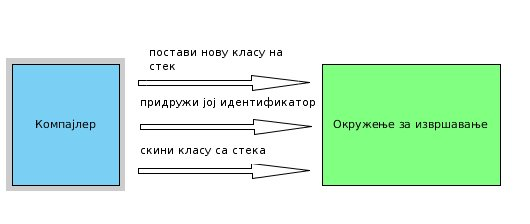
\includegraphics[width=0.8\textwidth]{compiler.jpg}
  \caption{Слање порука ЈИТ компилатора окружењу за извршавање.}
  \label{fig:komunikacija}
\end{figure}

Сва комуникација се врши преко одговарајућих протокола који се обично базирају на TCP/IP протоколу, чиме је омогућено удаљено извршавање. На овај начин велики део посла се пребацује на компилатор, а окружење за извршавање се максимално упрошћава.

Помоћу протокола за комуникацију компилатора и окружења за извршавање, може се постављати и мењати структура програма \cite{Dartino}.
Постављање структуре програма обухвата додавање нових класа и метода на стек окружења за извршавање.
Мењање структуре програма обухвата:
\begin{description}
\item Мењање табела метода\\
Омогућена је висока интерактивност са системом, што подразумева мењање понашања програма у току извршавања, нпр. додавањем новог метода класи, у одређеном тренутку. Компилатор ће окружењу за извршавање затражити да се промени табела метода.
\item Мењање шема\\
Мењање шема се односи на мењање класе, нпр.~додавањем нових поља. Оно што се дешава у тој ситуацији је да се врши пролаз кроз све инстанце класе, и оне се ажурирају и прилагођавају новом формату класе.
\item Дебаговање

У оквиру дебаговања, могуће је \cite{Dartino}:
\begin{enumerate}
\item Покретање дебагера
\item Постављање зауставних тачака
\item Рестартовање дебагера
\end{enumerate}
Систем за дебаговање је једноставан и ограничен, јер не зна ништа о изворном коду.
\end{description}
\section{Софтверска архитектура система}
\label{arhitektura}

Доњи слој софтверске архитектуре система са уграђеним рачунаром чини традиционални оперативни у реалном времену (нпр. Фри РТОС). Изнад тога се налази Дартино окружење за извршавање, које може извршавати више програма, независно, и они не морају знати ништа једни о другима. Ово се разликује од уобичајених система који раде на оперативном систему уграђеног рачунара, и који обично не могу да извршавају више независних компоненти, на независан начин. За сваки програм можемо имати више процеса, више инстанци програма, или делова програма, који се извршавају конкурентно \cite{Dartino}.

\begin{figure}[!ht]
  \centering
  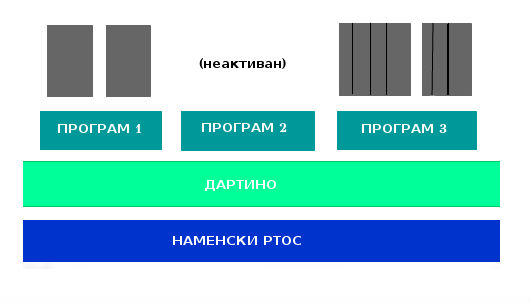
\includegraphics[width=0.7\textwidth]{arhitektura.jpg}
  \caption{Приказ софтверске архитектуре система, на примеру случаја када имамо више програма који се извршају конкурентно.}
  \label{fig:model}
\end{figure}
На слици \ref{fig:model} је приказана ситуација када имамо 3 програма. Програм2 се тренутно не извршава, за Програм1 су покренуте две инстанце, док се Програм3  извршава у 7 нити.

\section{Процеси и врсте процеса}
\label{procesi}
Дартино виртуелна машина има подршку за различите врсте процеса. Основни процеси су лаки процеси, али поред њих ту су влакна и изолате \cite{Dartino, procesi_i_izolate, korutine_i_vlakna}.
\subsection{Лаки процеси}
\label{laki_procesi}
За сваки процес нам је потребно мало меморије, неколико стотина бајтова. Сав к\^{о}д и подаци у меморији се деле, па меморију заузимају само подаци који представљају процес. На овај начин ради већина оперативних система, али је то новина за оперативне системе са уграђеним рачунаром.

Процес се може блокирати, при чему се не заузимају ресурси, већ се главна нит враћа систему. Разлог за то је што у системима са уграђеним рачунаром обично имамо мали фиксирани број нити, па не желимо да их блокирамо. 

Уколико процесор има више језгара, постоји подршка за паралелно извршавање нити које одговарају језгрима (енг.~\textit{native thread}). На сваком језгру се процеси извршавају конкурентно, а Дартино веома добро распоређује велики број процеса на много мањи број језгара \cite{Dartino}.

\begin{listing}
\begin{minted}[bgcolor=olive!10]{javascript}
main() {
  for (int i = 0; i < 4000; i++) {
    Process.spawn(hello(i));
  }
}
void hello(n) {
  print("Hello from \${i}");
}
\end{minted}
\caption{Креирање паралелних процеса методом \texttt{Process.spawn}.}
\label{paralelniprocesi}
\end{listing}

К\^{о}д \ref{paralelniprocesi} приказује покретање 4000 независних процеса за исписивање поздравне поруке, који ће бити распоређени на одређени број језгара и извршавати се паралелно. Сваки процес има своју хип меморију, а са осталим процесима може комуницирати само слањем порука. \textit{Process.spawn} креира нови процес и покреће га \cite{procesi_i_izolate}.

\begin{listing}
\begin{minted}[bgcolor=olive!10]{javascript}
var server = new ServerSocket("127.0.0.1", 0);
while(true) {
  server.spawnAccept((Socket socket){
	//izvrsava se u novom procesu
	socket.send(UTF.encode("Hello"));
	socket.close();
  })
}
\end{minted}
\caption{Манипулисање надолазећим конекцијама методом \texttt{spawnAccept}.}
\label{konekcije}
\end{listing}

У коду \ref{konekcije} се креира ServerSocket који представља сервер, затим се помоћу метода \textit{spawnAccept} креира нови процес. У оквиру тог процеса се чека да клијент успостави конекцију са сервером, и самим тим блокира даље извршавање док се конекција не успостави. При успостављању конекције, клијент (\textit{socket}) шаље серверу (\textit{server}) поздравну поруку \cite{Dartino}. Издвајање комуникације у нови процес је потребно вршити увек када се врши неко комплексније израчунавање пре слања поруке.

Комуникација између процеса се обавља слањем порука, помоћу канала и портова. Канал представља један ред порука. Порт представља могућност слања поруке каналу, и без приступа одеђеном порту, не може се слати порука каналу који чека на другој страни порта \cite{Dartino}.

\begin{listing}
\begin{minted}[bgcolor=olive!10]{javascript}
final channel = new Channel();
final port = new Port(channel);
Process.spawn(() {
	int i=0;
	while(i < 50) {
		port.send(i++);
	}
});
while(true) {
	print(channel.receive());
}
\end{minted}
\caption{Комуникација процеса слањем порука на одређени канал.}
\label{blokiranje}
\end{listing}

К\^{о}д \ref{blokiranje} приказује један процес који шаље поруке, и функцију \textit{print} која блокира извршавање све док не прими следећу поруку и испише је.

Процеси деле само објекте који се не мењају, и то на следећи начин \cite{Dartino}:
\begin{enumerate}
\item Сваки непроменљиви објекат се може слати као порука, без копирања
\item Више процеса могу користити(читати) исти објекат истовремено
\item Нема потребе за експлицитним примитивама за синхронизацију, јер мењање објеката није омогућено
\end{enumerate}

\subsection{Изолате}

Изолате су независни воркери, свака изолата има своју хип меморију, и за разлику од нити нема дељења меморије између изолата. Изолате комуницирају само преко порука. Могу се паузирати, наставити и убити \cite{procesi_i_izolate}. Детаљније су описане у поглављу \ref{dart_izolate}.

\subsection{Влакна}
\label{vlakna}

Влакна (енг.~\textit{Fibers}) представљају нити извршавања у оквиру једног процеса, које не деле непроменљиву меморију. Међутим, могу делити екстерну меморију (нпр.~помоћу класе ForeignMemory \footnote{https://dartino.github.io/api/dart-dartino.ffi/ForeignMemory-class.html.}), али се у том случају мора ручно водити рачуна о синхронизацији. Извршавају се конкурентно, тако да нема паралелизма. Омогућују да више независних нити једног процеса могу чекати на исту ствар(блокирати) независно једна од друге. На овај начин се могу имплементирати више одвојених контрола тока извршавања програма \cite{korutine_i_vlakna}.

\begin{listing}
\begin{minted}[bgcolor=olive!10]{javascript}
void publishOnChange(Socket socket, String property, Channel input){
  	 int last = 0;
  	 while(true){
   	  int current = input.receive();
    	 if(current != last)
      	 socket.send(UTF.encode('("\$property": \$current)'));
    	 last = current;
  	 }
}

Fiber.fork(() => publishOnChange(server, "temperature", tempSensor));
Fiber.fork(() => publishOnChange(server,"humidity", humSensor));
\end{minted}
\caption{Пример употребе два влакна која чекају на функцију \texttt{publishOnChange}, при чему не зависе једно од другог.}
\label{fibers}
\end{listing}

К\^{о}д \ref{fibers} приказује употребу два влакна. У оквиру једног се чека на промену вредности у сензору за температуру, док се у оквиру другог чека на промену вредности у сензору за влажност ваздуха \cite{Dartino}. Функција \textit{publishOnChange} блокира извршавање док се у сензору за који је позвана не деси промена вредности. На овај начин је омогућено да се у оквиру једног процеса чека на више ствари, и нема паралелизма, већ се уколико дође до блокирања у једном влакну, прелази на извршавање следећег који је спреман за извршавање.

\section{Корутине}
\label{korutine}

Дартино има уграђену подршку за корутине. Корутине су објекти налик на функције, које могу вратити више вредности. Када корутина врати вредност, зауставља се на тренутној позицији, а њен стек извршавања се чува за касније покретање. Када врати последњу вредност, сматра се завршеном, и више се не може покретати  \cite{korutine_i_vlakna}.

Кодом \ref{coroutines} дат је пример употребе корутина. Функција Expect.equals пореди две вредности које су јој прослеђене као аргументи, и у случају неједнакости враћа грешку. При првом позиву корутине co(1), резултат ће бити 4. Овај резултат је враћен позивом Coroutine.yield(4). Након позива yield, корутина ће бити суспендована. Другим позивом корутине co(2), њено извршавање ће се наставити тамо где је стала. Позив Expect.equals(2, 2) ће вратити тачно, и извршавање корутине ће се завршити. Пошто није наведена повратна вредност, резултат ће бити null. Након тога се корутина сматра завршеном и не може се наставити.

\begin{listing}
\begin{minted}[bgcolor=olive!10]{javascript}
var co = new Coroutine((x) {
    Expect.equals(1, x);
    Expect.equals(2, Coroutine.yield(4));
});

Expect.equals(4, co(1));
Expect.isTrue(co.isSuspended);
Expect.isNull(co(2));
Expect.isTrue(co.isDone);
\end{minted}
\caption{Употреба корутина.}
\label{coroutines}
\end{listing}

\section{Динамичко отпремање метода}
\label{sec:otpremanje}

Динамичко отпремање метода (енг.~\textit{Dynamic dispatch}) се односи на позивање полиморфних метода класа, при чему се који метод треба позвати разрешава у фази извршавања, а не у фази превођења. Прави се табела отпремања, која се имплементира као низ, у који се сваки метод, сваке класе, смешта на своју позицију. Позиција метода у табели се рачуна помоћу редног броја класе и позиције метода. У току извршавања, на основу ове табеле се одлучују који метод треба позвати. Оно што је неопходно при добијању одређеног метода из табеле, је провера да ли је резултат заправо оно што нам треба. Уколико није, значи да тражени метод одређене класе не постоји. Загарантовано је константно време отпремања, и табела отпремања се израчунава пре извршавања, па представља део апликације \cite{Dartino}.

\begin{listing}
\begin{minted}[bgcolor=olive!10]{javascript}
class A {
  metod1();
}
class B extends A {
  metod2();
}
class C extends B {
  metod1();
}
class D extends A {
  metod3();
}
\end{minted}
\caption{Пример хијерархије класа помоћу ког се илуструје генерисање табеле отпремања метода.}
\label{dispatchTable}
\end{listing}

У коду \ref{dispatchTable} је представљено неколико класа којима се преклапају методи. Процес генерисања табеле отпремања је следећи: Класама редом придружимо бројеве: 0, 1, 2 и 3. Методима придружимо померај на мало компликованији начин: методу \textit{metod1}, који је дефинисан у највећем броју класа, придружимо померај 0, и он се смешта на почетак табеле. Методу \textit{metod2} придружимо померај 3, и методу \textit{metod3} придружимо 4. Померају морају бити јединствени бројеви, како не би дошло до преклапања метода \cite{Dartino}.

У наставку је пример рачунања позиције метода у табели отпремања:
\begin{itemize}
\item Позиција метода \textit{metod1} за класу А: 0 (редни број класе) + 0 (померај метода) = 0
\item Позиција метода \textit{metod1} за класу B: 1 (редни број класе) + 0 (померај метода) = 1
\item Позиција метода \textit{metod1} за класу C: 2 (редни број класе) + 0 (померај метода) = 2
\item Позиција метода \textit{metod1} за класу D: 3 (редни број класе) + 0 (померај метода) = 3
\item Позиција метода \textit{metod2} за класу B: 1 (редни број класе) + 3 (померај метода) = 4
\item Позиција метода \textit{metod2} за класу C: 2 (редни број класе) + 3 (померај метода) = 5
\item Позиција метода \textit{metod3} за класу D: 3 (редни број класе) + 4 (померај метода) = 7
\end{itemize}

Пример табеле отпремања за ове класе приказан је на слици \ref{fig:otpremanje}. Приметимо да се могу појавити празне позиције у табели.

\begin{figure}[!ht]
  \centering
  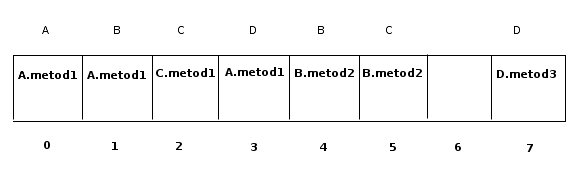
\includegraphics[width=0.7\textwidth]{otpremanje.jpg}
  \caption{Табела отпремања за класе у примеру \ref{dispatchTable}.}
  \label{fig:otpremanje}
\end{figure}

\section{Најзначајније библиотеке}
\label{biblioteke}
Ради прилагођавања програмског језика Дарт специфичностима микроконтролера, развијена је нова библиотека \textit{,,dartino''}. Она се састоји из више мањих библиотека, а неке од најзначајних су описане у наставку  \cite{biblioteke}.

\begin{description}

\item ~\textbf{file} - Интерфејс за рад са датотекама. Подржано само када се Дартино извршава на ПОСИКС платформи.

\item ~\textbf{ffi} - ,,foreign function interface'' библиотека која омогућава да се из Дарт кода позивају функције дефинисане у неком другом програмском језику, нпр. функције програмског језика Ц.

\item ~\textbf{http} - Имплементација ХТТП (енг.~\textit{HTTP - HyperText Transfer Protocol}) клијента.

\item ~\textbf{mbedtls} - ТЛС (енг.~\textit{TLS - Transport Layer Security}) подршка, базирана на mbedtls\footnote{ Имплементација ТЛС и ССЛ сигурносних протокола и одговарајућих алгоритама криптовања.} \cite{mbed}.
Ово се може користити на исти начин као нормални сокет (и да се прослеђује ХТТП пакету).

\item ~\textbf{mqtt} - MQTT клијентска библиотека за MQTT (скраћено од MQ Telemetry Transport) протокол, ИоТ протокол за размену порука заснован на објављивању/претплати \cite{mqtt}.

\item ~\textbf{os} - Приступ оператитивном систему. Подржано када се Дартино извршава на ПОСИКС платформи.

\item ~\textbf{socket} - Дартино имплементација ТЦП (енг.~\textit{TCP - Transmission Control Protocol}) и УДП (енг.~\textit{UDP - User Datagram Protocol}) сокета

\item ~\textbf{stm32} - Подршка за STM32\footnote{Фамилија микроконтролера базираних на 32-битним АРМ процесорима.} плоче.

\end{description}

\section{Покретање Дарт програма унутар виртуелне машине}
\label{sec:pokretanje}

Примарни начин за комуникацију са Дартино виртуелном машином је преко команде ~\textbf{dartino}. Ова команда комуницира са dart процесом, који се извршава у позадини и не захтева интеракцију са корисником (енг.~\textit{persistent process}). Дарт процес омогућава компилацију, док Дартино виртуелна машина (~\textbf{dartino-vm}) извршава и дебагује програме .\\

Нешто више о извршним фајловима које се користе при покретању програма \cite{komande}:
\begin{description}
\item ~\textbf{dartino}
Ово је мали извршни фајл који преко сокета прослеђује стандардне улазно/излазне сигнале процесу dart. Служи за покретање ЈИТ компилатора који je написан у Дарту и извршава се у оквиру Дарт виртуелне машине
\item ~\textbf{dartino-vm} 
Виртуелна машина која покреће програм из бајткода.
\item ~\textbf{dart}
dart је процес који се у позадини извршава и не захтева интеракцију са корисником. Овај процес се састоји од главне нити и неколико воркера. Главна нит ослушкује надолазеће конекције из ~\textbf{dartino} команде, и може да користи воркере да обави тражени задатак. Основна улога овог процеса је покретање Дарт компилатора. Овај процес се извршава на Дарт виртуелној машини.
\end{description}

Шта се заправо дешава када се покрене команда ~\textbf{dartino run hello.dart}? Дартино је подразумевано повезан на локалну сесију, која је повезана на локалну виртуелну машину која ради на нашем рачунару. ~\textbf{dartino} преводи к\^{о}д до бајткода, помоћу Дарт компилатора, а онда га прослеђује ~\textbf{dartino-vm} која га извршава. Дартино виртуелна машина враћа резултат назад Дартину, и он га приказује.

Дартино подржава више сесија. Свака сесија може бити придружена различитој Дартино виртуелној машини, што омогућује кориснику да тестира више разлићитих уређаја истовремено. Тренутно је руковање сесијама експлицитно \cite{Dartino, komande}.

\begin{figure}[!ht]
  \centering
  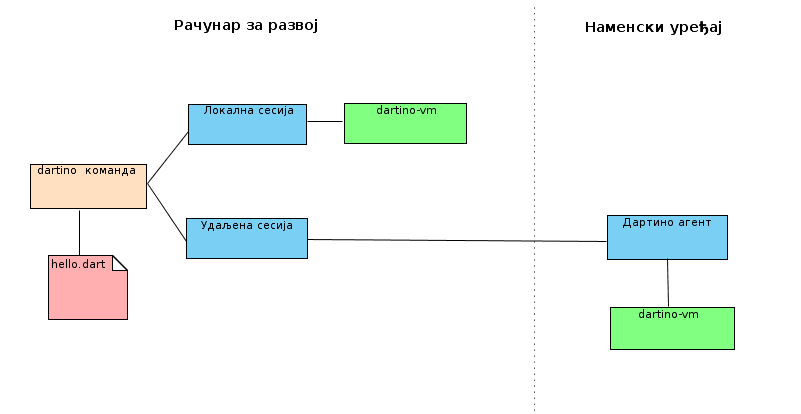
\includegraphics[width=0.9\textwidth]{sesije.png}
  \caption{Процес извршавања програма.}
  \label{fig:izvrsavanje}
\end{figure}

Покретање програма у оквиру одређене сесије је омогућено на следећи начин [6]:

~\textbf{./dartino create session my\_session}\\
Креирање нове сесије ,,my\_session''.

Након тога морамо да покренемо дартино виртуелну машину:

~\textbf{./dartino-vm}\\
Након покретања дартино виртуелне машине се исписује порука облика ,,Waiting for compiler on 127.0.0.1:61745'', при чему број 61745 представља рандом генерисани порт.

Да би се прикачили на дати сокет, потребно је да отворимо нови терминал и у њему покренемо dartino команду са наредним параметрима:

~\textbf{./dartino attach tcp\_socket 127.0.0.1:61745 in session my\_session}\\

Затим у оквиру те сесије можемо да покренемо жељени програм на следећи начин:

~\textbf{./dartino run hello.dart in session my\_session}\\

Сесија се прекида помоћу следеће команде:

~\textbf{./dartino x-end session my\_session}\\


% ------------------------------------------------------------------------------
\chapter{Имплементација интерпретатора за платформу МИПС}
\label{chp:implementacija}
% ------------------------------------------------------------------------------
У овој глави је описан поступак имплементације интерпретатора за платформу МИПС, кроз делове кода и одређене тест примере који су развијани у току имплементације. У поглављу \ref{sec:stek} је описан стек Дартино виртуелне машине, док је у поглављу \ref{sec:debagovanje} описан имплементирани систем за дебаговање. У поглављу \ref{testiranje} описани су још неки значајни тест примери, резултати тестирања на постојећем скупу тестова и програм у језику Дарт, имплементиран за потребе упоређивања перформанси интерпретатора.

\section{Имплементација у програмском језику Ц++}
Имплементација је рађена на рачунару са Интел x86 процесором, крос-компилацијом, при чему је циљна архитектура  МИПС32Р2 (енг.~\textit{mips32r2}, скраћено од mips32 release 2). Имплементирани интерпретатор генерише асемблерску датотеку чијим превођењем добијамо програм који извршава бајткод на МИПС архитектури.

У почетку развоја, постојао је мултинаменски интерпретатор, који не зависи од архитектуре. Било је потребно конфигурисати Дартино за платформу МИПС, и на тај начин обезбедити превођење за МИПС платформу. 

У наставку ће бити описан процес превођења Дартино виртуелне машине, и шта све обухвата конфигурисање за МИПС.
Превођење се врши помоћу \textit{ninja} система за превођење. Ово је мали, веома брз систем за превођење, који се обично не пише ручно. Како је једини циљ при имплементацији овог система била брзина, он је читљив, али се препоручује коришћење у комбинацији са другим мета системима за превођење. У оквиру Дартино пројекта коришћен је \textit{gyp} мета систем. Превођење се врши командом \textit{ninja} која у оквиру текућег директоријума тражи датотеку \textit{build.ninja}. Ова датотека се генерише на основу одговарајућих \textit{.gyp} и \textit{.gypi} датотека. 

У датотеци \textit{default\_targets.gypi} дефинишу се подржане архитектуре. За МИПС је потребно додати \textit{DebugXMIPS} (X-означава се врши крос-компилација). Овде се за сваку од архитектура увлачи конфигурација из датотеке \textit{common.gypi}. У датотеци \textit{common.gypi} дефинише се у којим датотекама се врши покретање одређене врсте ГЦЦ-а и Г++-a. То су датотеке \textit{cc\_wrapper.py} и \textit{cxx\_wrapper.py}. Поред тога, у \textit{common.gypi} су дефинисани флегови који се прослеђују ГЦЦ-у, који су независни од архитектуре. Такође, овде се дефинише и врста оперативног система. Затим се за сваку од архитектура дефинишу одговарајући флегови, као и путање до библиотека које се користе у фази линковања. За МИПС је потребно навести \textit{'-mips32r2'} који означава циљну архитектуру и \textit{'-EL'} што указује да је запис података у меморији такав да је на нижој адреси нижи бит меморијске речи (енг.~\textit{little endian}). Поред тога, потребно је навести путање до библиотека које се налазе у оквиру одређеног ланца алата за МИПС (енг. \textit{mips toolchain}). Такође, за сваку од архитектура, дефинишу се ,,лажни'' макрои који се користе у датотекама \textit{cc\_wrapper.py} и \textit{cxx\_wrapper.py}, како би се на основу њих изабрао одређени скуп алата који се користи при превођењу, а након тога се ти макрои пониште. Ови макрои су ,,лажни'' јер се прослеђују заједно са флеговима који се користе у фази линковања, али се избаце из тог скупа пре него што дођу до линкера. За платформу МИПС, у оквиру датотека \textit{cc\_wrapper.py} и \textit{cxx\_wrapper.py} треба додати да се покрећу ГЦЦ и Г++ из одређеног ланца алата за МИПС.

На овај начин је омогућено покретање команде \textit{ninja} која врши превођење и креира одговарајуће излазне (енг.~\textit{out}) директоријуме за сваку од подржаних архитектура. Након тога је потребно извршити превођење за жељену архитектуру. Превођење за МИПС врши се помоћу команде \textit{ninja -C out/DebugXMIPS}.

МИПС извршне датотеке се покрећу помоћу КЕМУ (енг.~\textit{QEMU - Quick Emulator}) емулатора у корисничком режиму\footnote{У овом режиму КЕМУ може покретати процесе преведене за једну врсту процесора на другој врсти процесора.}. Да би се то вршило аутоматски, непходно је линукс команди \textit{update-binfmts} проследити вредности које одговарају мипс ЕЛФ (енг.~\textit{ ELF - format of Executable and Linking Format} \footnote{Бинарни формат извршних датотека на Линукс оперативном систему.}) датотекама, и путању до скрипте која покреће КЕМУ емулатор. Верзија 2.1.43 линукс кернела, и све након ње, садрже \textit{binfmt\_misc} модул. Овај модул омогућује да системски администратор може регистровати који се интерпретатор треба користити за различите бинарне формате, на основу магичних вредности и вредности маске (енг.~\textit{magic and mask}), и да при регистровању датотеке која има те вредности, позове одговарајући интерпретатор. Команда \textbf{update-binfmts} управља базом ових интерпретатора. Команда са одговарајућим аргументима је представљена кодом \ref{qemu_komanda}, док је скрипта која покреће КЕМУ представљена кодом \ref{skripta}. \\

\begin{listing}
\centering
\begin{minted}[bgcolor=olive!10]{awk}
sudo update-binfmts --install qemu-mipsel /<skripta>
--magic '\x7fELF\x01\x01\x01\x00\x00\x00\x00
        \x00\x00\x00\x00\x00\x02\x00\x08\x00'
--mask '\xff\xff\xff\xff\xff\xff\xff\x00\xfe\xff
        \xff\xff\xff\xff\xff\xff\xfe\xff\xff\xff'
--credentials yes --package qemu-user-static
\end{minted}
\caption{Команда за аутоматско покретање МИПС извршних датотека помоћу КЕМУ-a. <skripta> представља путању до скрипте \ref{skripta}.}
\label{qemu_komanda}
\end{listing}


\begin{listing}
\centering
\begin{minted}[bgcolor=olive!10]{awk}
#!/bin/bash
qemu=/<qemu>/mipsel-linux-user/qemu-mipsel
exec $qemu $*
\end{minted}
\caption{Скрипта у којој се покреће КЕМУ емулатор. <qemu> представља путању до директоријума у ком се налази КЕМУ емулатор.}
\label{skripta}
\end{listing}

Имплементација је рађена у програмском језику Ц++. Пре имплементације интерпретатора, направљене су датотеке \textit{assembler\_mips.h},  \textit{assembler\_mips.cc} и \textit{assembler\_mips\_linux.cc} које описују МИПС асемблерски језик. У датотеци \textit{assembler\_mips.h} дефинисана је енумерација регистра која обухвата МИПС регистре. Више о МИПС регистрима речено је у поглављу \ref{sec:registers}. Направљене су класе \textit{Label}, \textit{Constant} и \textit{Address}. 

\begin{listing}
\begin{minted}[bgcolor=olive!10]{cpp}
class Label {
 public:
  Label() : position_(-1) {}

  int position() {
    if (position_ == -1) position_ = position_counter_++;
    return position_;
  }

 private:
  int position_;
  static int position_counter_;
}; 
\end{minted}
\caption{Класа помоћу које се генеришу лабеле у МИПС асемблерском језику.}
\label{label}
\end{listing}

Лабела представља линију у оквиру асемблерског фајла на коју се може скочити. У коду \ref{label} је представљена класа \textit{Label} која садржи два поља: \textit{position} - представља редни број лабеле и \textit{position\_counter} - заједничка променљива за све инстанце класе \textit{Label}, на основу које се додељује позиција лабеле.\\

\begin{listing}
\begin{minted}[bgcolor=olive!10]{cpp}
class Immediate {
 public:
  explicit Immediate(int32_t value) : value_(value) {}
  int32_t value() const { return value_; }

 private:
  const int32_t value_;
};
\end{minted}
\caption{Класа помоћу које се генеришу константе у МИПС асемблерском језику.}
\label{konstanta}
\end{listing}

У коду \ref{konstanta} је представљена класа \textit{Immediate}. Инстанца те класе представља константу вредност целобројног типа.\\

\begin{listing}
\begin{minted}[bgcolor=olive!10]{cpp}
class Address {
 public:
  Address(Register base, int32_t offset)
      : base_(base), offset_(offset) {}

  Register base() const { return base_; }
  int32_t offset() const { return offset_; }

 private:
  const Register base_;
  const int32_t offset_;
};
\end{minted}
\caption{Класа помоћу које се представљају меморијске адресе у МИПС асемблерском језику.}
\label{adresa}
\end{listing}

У коду \ref{adresa} је представљена класа \textit{Address}. Инстанца те класе представља меморијску адресу, која је на платформи МИПС32Р2 32-битна. Адреса се рачуна као збир адресе у базном регистру и помераја. Базни регистар је регистар опште намене који садржи 32-битну адресу. 

Дефинисани су макрои за МИПС инструкције са одговарајућим бројем аргумената. Помоћу ових макроа, у оквиру класе \textit{Assembler} дефинисане су све МИПС инструкције које су потребне при интерпретацији.\\

\begin{listing}
\begin{minted}[bgcolor=olive!10]{cpp}
#define INSTRUCTION_3(name, format, t0, t1, t2)  \
  void name(t0 a0, t1 a1, t2 a2) {               \
    Print(format, Wrap(a0), Wrap(a1), Wrap(a2)); \
  }
\end{minted}
\caption{Макро за генерисање инструкције која има 3 аргумента.}
\label{instrukcija}
\end{listing}

У коду \ref{instrukcija} представљен је пример макроа за генерисање МИПС асемблерских инструкција које имају 3 аргумента. Аналогно томе, постоје макрои за генерисање инструкција са 1, 2 и 4 аргумента.

У оквиру класе \textit{Assembler} имплементиране су методе \textit{SwitchToText()} и \textit{SwitchToData()} које постављају директиве за сегмент података, односно кодни сегмент. Поред тога, класа \textit{Assembler} садржи и методе који представљају ,,псеудоинструкције'' генерисане ради прегледанијег кода. Нпр. метод \textit{B} представља ,,псеудоинструкцију'' која врши гранање и након тога попуњава слот закашњења инструкцијом \textit{nop}. 
У оквиру ове класе је имплементирана и функција \textit{Print} за уписивање асемблерских инструкција у фајл. Дефинисан је начин записивања регистара, лабела и адреса у МИПС асемблеру.\\

\begin{listing}
\begin{minted}[bgcolor=olive!10]{cpp}
case 'l': {
  Label* label = va_arg(arguments, Label*);
  printf(".L%d", label->position());
  break;
}
\end{minted}
\caption{Пример записивања лабеле у МИПС асемблерском језику.}
\label{print_labela}
\end{listing}

У коду \ref{print_labela} представљен је део функције \textit{Print} који се односи на начин записивања лабеле унутар асемблерског фајла. Пре позиције додаје се префикс ,,.L'' који означава да је у питању лабела.

\begin{listing}
\begin{minted}[bgcolor=olive!10]{cpp}
case 'r': {
  Register reg = static_cast<Register>(va_arg(arguments, int));
  printf("\$%s", ToString(reg));
  break;
 }
\end{minted}
\caption{Пример записивања регистра у МИПС асемблерском језику.}
\label{print_registar}
\end{listing}
У коду \ref{print_registar} представљен је део функције \textit{Print} који се односи начин записивања регистра унутар асемблерског фајла. Регистар се означава префиксом ,,\$'', након чега следи ознака регистра.

\begin{listing}
\begin{minted}[bgcolor=olive!10]{cpp}
void Assembler::PrintAddress(const Address* address) {
  printf("\%d(\$%s)", address->offset(), ToString(address->base()));
}
\end{minted}
\caption{Пример записивања адресе у МИПС асемблерском језику.}
\label{print_adresa}
\end{listing}
У коду \ref{print_adresa} представљен је део функције \textit{Print} који се односи начин записивања адресе унутар асемблерског фајла. Адреса се записује као померај иза ког следи у загради запис базног регистра.


На овај начин је омогућено генерисање МИПС асемблерског кода. 

У оквиру интерпретатора имплементиране су класе \textit{InterpreterGenerator} и \textit{InterpreterGeneratorMIPS}. Класа \textit{InterpreterGenerator} је апстрактна. У оквиру ње је имплементиран метод \textit{Generate} који је одговорaн за генерисање асемблерског кода. Класа као једини приватни податак чува \textit{assembler}.

Класа дефинише макро \textit{V(name, branching, format, size, stack\_diff, print)} који се користи за генерисање виртуелних апстрактних метода који имају потпис \textit{void Do\#\#name()}. У оквиру овог макроа, позива се макро \textit{BYTECODES\_DO(V)} који је дефинисан у датотеци \textit{bytecodes.h}. У њему се позива макро \textit{V(name, branching, format, size, stack\_diff, print)} за све методе тог формата. Неке од тих метода су \textit{DoLoadLocal}, \textit{DoLoadField}, \textit{DoLoadLiteralTrue} итд. Слично томе дефинише се и макро \textit{V(name)}.

У оквиру метода \textit{Generate} позивају се виртуелни апстрактни методи \textit{GeneratePrologue}, \textit{GenerateEpilogue}, \textit{GenerateMethodEntry}, \textit{GenerateBytecodePrologue} и \textit{GenerateDebugAtBytecode}. Методи \textit{GeneratePrologue}, \textit{GenerateEpilogue} односе се на МИПС позивну конвенцију, која је описана у поглављу \ref{konvencija}. Функција \textit{GeneratePrologue} служи за генерисање асемблерског кода који ће се извршити приликом позива сваке функције. Мора се сачувати садржај регистара \textit{\$s0-\$s7} на стеку, и такође садржај регистра \textit{\$ra}, у ком се налази адреса повратка функције. По повратку из неке функције, позива се функција \textit{GenerateEpilogue} у којој се скида са стека садржај регистара \textit{\$s0-s7} и регистра \textit{\$ra}.

Поред тога, у оквиру метода \textit{Generate} дефинише се макро \textit{V(name, branching, format, size, stack\_diff, print)} помоћу ког се позивају већ наведени методи (\textit{DoLoadField}, \textit{DoLoadLiteralTrue} итд). Пре позива сваког од метода, позива се метод који генерише одговарајућу лабелу у оквиру асемблерске датотеке, како би се на део кода који генерише тај метод могло скочити. На сличан начин се дефинише макро \textit{V(name)}, помоћу ког се позивају методи дефинисани макроом \textit{V(name)}. Такође, у оквиру метода \textit{Generate}, у сектору података се декларишу лабеле на које се може скочити.

Након дефиниције класе, позива се макро \textit{GENERATE(, Interpret)}. Овај макро је дефинисан у датотеци \textit{generator.h}. У њему се дефинише функција која позива метод \textit{Generate} класе \textit{InterpreterGeneratorMIPS}. Помоћу те функције се генерише асемблерски код.

Класа \textit{InterpreterGeneratorMIPS} наслеђује класу \textit{InterpreterGenerator} и имплементира све њене виртуелне методе. 
Од приватних података, ова класа садржи лабеле помоћу којих се означавају делови кода на које се може скакати из различитих метода. Неке од тих лабела су \textit{check\_stack\_overflow}, помоћу које се скаче на део кода који врши проверу прекорачења на стеку, и \textit{done\_} лабела која се користи за скакање на део кода који сачува садржаје регистара на стеку.

У оквиру ове класе дефинише се макро \textit{INVOKE\_BUILTIN(kind)}, помоћу ког се деклараришу методи који имају исти потпис, облика \textit{DoInvoke\#\#kind()} и облика \textit{DoInvoke\#\#kind\#\#Unfold()}. То су методи који имплементирају поређење (нпр~\textit{DoInvokeЕq}), методи који имплементирају основне аритметичке операције (нпр.~\textit{DoInvokeAdd}), и методи који имплементирају битовске операторе (нпр.~\textit{DoInvokeBitNot}). Поред тога, ова класа имплементира и све остале виртуелне апстрактне методе своје надкласе. Међу тим методама се налазе методи за учитавање локалних података, нпр. метод \textit{LoadLocal0} који учитава садржај са врха стека у регистар \textit{\$a0}, а затим тај регистар сачува на стеку. Ови методи се користе за прослеђивање аргумената функцији која се позива. Такође, међу имплементираним методама су методи који се односе на гранање, методи који се односе на избацивање изузетака, методи за рад са корутинама, методи за поређење. ПОТРЕБНО ЈЕ БОЉЕ ГРУПИСАТИ СВЕ МЕТОДЕ И ОПИСАТИ ИХ

При скоку на функцију која се налази ван интерпретатора, мора се позвати метод за поравнање стека. Овај метод је представљен кодом \ref{prepare_stack}. На основу позивне конвенције, описане у поглављу \ref{konvencija}, неопходно је резервисати 4 места на стеку за аргументе функције (уколико функција коју позивамо позива неку другу функцију). Осим тога, неопходно је сачувати садржај регистра \textit{\$gp}. Стек увек мора бити поравнат на 8 (адреса стека мора бити дељива са 8), па се због тога сачува 6 речи уместо 5.\\

\begin{listing}
\begin{minted}[bgcolor=olive!10]{javascript}
void InterpreterGeneratorMIPS::PrepareStack() {
  __ addiu(SP, SP, Immediate(-6 * kWordSize));
  __ sw(GP, Address(SP, 5 * kWordSize));
}
\end{minted}
\caption{Пример метода за поравнање стека, која се позива пре скока на неку спољну функцију.}
\label{prepare_stack}
\end{listing}

По повратку из неке спољне функције, позива се метод \textit{RestoreStack}, која ради инверзну операцију метода \textit{PrepareStack}. Овај метод је представљен кодом \ref{restore_stack}.\\

\begin{listing}
\begin{minted}[bgcolor=olive!10]{javascript}
void InterpreterGeneratorMIPS::RestoreStack() {
  __ lw(GP, Address(SP, 5 * kWordSize));
  __ addiu(SP, SP, Immediate(6 * kWordSize));
}
\end{minted}
\caption{Пример метода за поравнање стека, која се позива по повратку из неке спољне функцију.}
\label{restore_stack}
\end{listing}

Кодом \ref{function_add} представљена је функција која сабира два броја, при чему се проверава да ли је дошло до прекорачења. Уколико је било прекорачења, непходно је скочити на део кода који врши опоравак.\\

\begin{listing}
\begin{minted}[bgcolor=olive!10]{cpp}
void InterpreterGeneratorMIPS::InvokeAdd(const char* fallback) {
  Label no_overflow;
  LoadLocal(A0, 1);
  __ andi(T0, A0, Immediate(Smi::kTagMask));
  __ B(NEQ, T0, ZR, fallback);
  LoadLocal(A1, 0);
  __ andi(T1, A1, Immediate(Smi::kTagMask));
  __ B(NEQ, T1, ZR, fallback);

  __ xor_(T1, A0, A1);
  __ b(LT, T1, ZR, &no_overflow);
  __ addu(T0, A0, A1);  // Delay-slot.
  __ xor_(T1, T0, A0);
  __ b(LT, T1, ZR, fallback);
  __ Bind(&no_overflow);
  __ move(A0, T0);  // Delay-slot.
  DropNAndSetTop(1, A0);
  Dispatch(kInvokeAddLength);
}
\end{minted}
\caption{Функција у МИПС интерпретатору која сабира две целобројне вредности.}
\label{function_add}
\end{listing}

Први програм који је успешно извршен помоћу МИПС интерпретатора био је програм који декларише променљиву и иницијализује је на вредност 42, а затим је исписује на стандардни излаз. Овај програм је представљен кодом \ref{return_42}.\\

\begin{listing}
\begin{minted}[bgcolor=olive!10]{javascript}
main() {
  var number = 42;
  print(\${number});
}
\end{minted}
\caption{Прoграм за исписивање броја 42 у програмском језику Дарт.}
\label{return_42}
\end{listing}

Како би се омогућило дебаговање интерпретатора, направљен је механизам за дебаговање у МИПС асемблеру који садржи две опције: могућност исписивања редног броја функције интерпретатора која се тренутно извршава и могућност исписивања садржаја задатог регистра. Ти механизми су у процесу развоја били део интерпретатора. Када дође до грешке и прекида извршавања програма, овај механизам нам омогућава да знамо у којој функцији је дошло до грешке. Овај механизам је детаљније описан у поглављу \ref{sec:debagovanje}.

Други програм који је успешно извршен помоћу МИПС интерпретатора је програм који исписује поздравну поруку. Овај програм је представљен кодом \ref{hello_world}.\\

\begin{listing}
\begin{minted}[bgcolor=olive!10]{javascript}
main() {
  print("Hello world");
}
\end{minted}
\caption{Прoграм за исписивање поруке "Hello world" у програмском језику Дарт.}
\label{hello_world}
\end{listing}

Први програм из подржаног скупа тестова, који је покренут помоћу МИПС интерпретатора, је  програм који исписује поздравну поруку и информације о машини на којој се извршава. Овај програм представљен је кодом \ref{hello_from}.\\

\begin{listing}
\begin{minted}[bgcolor=olive!10]{cpp}
main() {
  SystemInformation si = sys.info();
  String nodeInformation =
      si.nodeName.isEmpty ? '' : ' running on \${si.nodeName}';
  print('Hello from ${si.operatingSystemName}$nodeInformation.');
}
\end{minted}
\caption{Програм који исписује ,,Hello'' и информације о машини на којој се извршава.}
\label{hello_from}
\end{listing}

Више о тестирању речено је у поглављу 

\section{Дартино стек}
\label{sec:stek}

У оквиру Дартино виртуелне машине се ради са локалним стеком, и за те потребе је искоришћен регистар \textit{\$s2}. Све операције са стеком у оквиру интерпретатора се раде над тим стеком, при чему стек процесора користи Дарт виртуелна машина, односно компајлер.
Функције која врши скидање садржаја са стека је представљена кодом \ref{pop}. У регистар се упише садржај са врха стека, а затим се врх стека помери за дужину једне речи, односно садржај се скине са стека.
Функција која поставља садржај на стек је представљена кодом \ref{push}. На стеку се алоцира меморија за једну реч (помери се врх стека), а затим се садржај регистра упише на врх стека.\\

\begin{listing}
\begin{minted}[bgcolor=olive!10]{cpp}
void InterpreterGeneratorMIPS::Pop(Register reg) {
  __ lw(reg, Address(S2, 0));
  __ addiu(S2, S2, Immediate(1 * kWordSize));
}
\end{minted}
\caption{Функција за скидање садржаја регистра са локалног Дартино стека.}
\label{pop}
\end{listing}

\begin{listing}
\begin{minted}[bgcolor=olive!10]{cpp}
void InterpreterGeneratorMIPS::Push(Register reg) {
  __ addiu(S2, S2, Immediate(-1 * kWordSize));
  __ sw(reg, Address(S2, 0));
}
\end{minted}
\caption{Функција за чување садржаја регистра на локалном Дартино стеку.}
\label{push}
\end{listing}

\section{Систем за дебаговање}
\label{sec:debagovanje}
Како се у току превођења Дартина, од интерпретатора генерише асемблерска датотека, која се затим се користи за генерисање програма који извршава бајткод на МИПС архитектури, било је неопходно да се систем за дебаговање угради у асемблерски код.

У коду \ref{push_asm} представљен је макро у оквиру ког се налазе инструкције за чување садржаја регистра на стеку. Чување садржаја на стеку је имплементирано као у функцији која је представљена кодом \ref{push}, при чему је једина разлика то што се ради са процесорским стеком.

У коду \ref{pop_asm} представљене су инструкције за скидање садржаја регистра на стеку. Макро је имплеметиран исто као функција у коду \ref{pop}. 

\begin{listing}
\begin{minted}[bgcolor=olive!10]{cpp}
#define push_asm(reg)                               \
  assembler()->subi(SP, SP, Immediate(1*kWordSize));\
  assembler()->sw(reg, Address(SP, 0));
\end{minted}
\caption{Макро за чување садржаја регистра са стека.}
\label{push_asm}
\end{listing}

\begin{listing}
\begin{minted}[bgcolor=olive!10]{cpp}
#define pop_asm(reg)                                \
  assembler()->lw(reg, Address(SP, 0));             \
  assembler()->addi(SP, SP, Immediate(1*kWordSize));
\end{minted}
\caption{Макро за скидање садржаја регистра са стека.}
\label{pop_asm}
\end{listing}

\begin{listing}
\begin{minted}[bgcolor=olive!10]{cpp}
#define PrintRegister(reg)                      \
  push_asm(GP);                                 \
  push_asm(V0);                                 \
  push_asm(A0);                                 \
  push_asm(A1);                                 \
  push_asm(T9);                                 \
  push_asm(RA);                                 \
  assembler()->la(A0, "print_reg");             \
  assembler()->move(A1, reg);                   \
  assembler()->lw(T9, "\%call16(printf)(\$gp)");\
  assembler()->jalr(T9);                        \
  assembler()->nop();                           \
  pop_asm(RA);                                  \
  pop_asm(T9);                                  \
  pop_asm(A1);                                  \
  pop_asm(A0);                                  \
  pop_asm(V0);                                  \
  pop_asm(GP);                                  
\end{minted}
\caption{Макро за исписивање садржаја регистра.}
\label{print_reg}
\end{listing}

У коду \ref{print_reg} приказан је макро који се користи да би се исписао садржај регистра. Неопходно је сачувати садржај регистара који се користе у макроу, како систем за дебаговање не би утицао на извршавање остатка програма. У \textit{\$a0} се смешта адреса ниске "print\_reg", коју генерише функција \textit{GenerateDebugStrings} док се у \textit{\$a1} сачува садржај регистра који је аргумент макроа. Након тога се скочи на функцију \textit{printf}, при чему се у \textit{\$a0} и \textit{\$a1} налазе аргументи функције. Сличан макро генерисан је за записивање редног броја функције интерпретатора која се тренутно извршава.\\

\begin{listing}
\begin{minted}[bgcolor=olive!10]{cpp}
void InterpreterGeneratorMIPS::GenerateDebugStrings() {
  int i;
  char *str = (char *)malloc(10);
  printf("\n\t.data\n");
  for(i=1;i<=255;i++) {
    sprintf(str, "string_\%d", i);
    printf("\%s: .asciiz \"\%d   \"\n", str, i);
  }
  printf("print_reg: .asciiz \"register_value: \%\%x\\n\"\n");
  free(str);
}
\end{minted}
\caption{Функција која генерише ниске које се користе при дебаговању, у сектору података у асемблерској датотеци.}
\label{generate_debug_strings}
\end{listing}

У коду \ref{generate_debug_strings} приказана је функција која се користи при генерисању ниски које се користе при дебаговању: ,,string\_редни\_број\_ниске'' и ,,print\_reg''. Ниска  ,,string\_редни\_број\_ниске'' представља лабелу која се записује у сектору података, иза које следи ,,.asciiz'', што представља тип податка, и на крају сам податак, односно број. Ова ниска се користи у интерпретатору при исписивању редног броја функције која се тренутно извршава.
Ниска ,,print\_reg'' користи се при исписивању садржаја регистра, што је приказано кодом \ref{print_reg}. Ова ниска такође представља лабелу у сектору података, иза које следи тип ,,.asciiz'', и на крају вредност податка, односно садржај регистра који се исписује. Више о запису у сектору података у МИПС асемблерском језику описано је у поглављу \ref{struktura}.

\section{Тестирање и резултати}
\label{testiranje}
Упоредо са имплементацијом интерпретатора, писани су мали тест примери. Примери неких тестова дати су у опису имплементације. Овде ће бити наведени још неки од тестова који су помогли у решавању највећих багова.

Један од проблема који се јавио у току имплементације је функција \textit{signalfd}, која у КЕМУ емулатору за МИПС није била имплементирана. То је установљено тест примером који је приказан кодом \ref{signal_fd}.\\

\begin{listing}
\begin{minted}[bgcolor=olive!10]{cpp}
int fd = signalfd(-1, &signal_mask, SFD_CLOEXEC);
  if (fd == -1) {
    FATAL1("signalfd failed: %s", strerror(errno));
  }
\end{minted}
\caption{Позив функције \texttt{signalfd}, који је производио грешку при извршавању.}
\label{signal_fd}
\end{listing}

Након тога је направљен тест у програмском језику Ц, у ком се такође користи функција \textit{signalfd}, и преведен за МИПС, како би се утврдило да ли разлог због ког не пролази тест има везе са интерпретатором. При извршавању тог теста јављала се грешка неподржане функције. Kaда je подршка за функцију додата у оквиру КЕМУ емулатора, тест је прошао.

Приликом тестирања рада са сокетима јавила се грешка при позиву функције \textit{Socket.connect}, односно функције \textit{sys.socket} која се налази у оквиру ње. Пример позива те функције дат је кодом \ref{sys.socket}.\\

\begin{listing}
\begin{minted}[bgcolor=olive!10]{cpp}
fd = sys.socket(sys.AF_INET, sys.SOCK_STREAM, 0);
\end{minted}
\caption{Позив функције \texttt{sys.socket}, који је производио грешку при извршавању.}
\label{sys.socket}
\end{listing}

Утврђено је да унутар Дартина вредност макроа \textit{SOCK\_STREAM} није прилагођена МИПС архитектури, која користи различите вредности неких системских макроа у односу на остале архитектуре.

Направљено је и неколико тест примера у којима је уочен проблем при позиву функције \textit{sys.setsockopt}, којој су прослеђиване погрешне вредности макроа \textit{SOL\_SOCKET} и \textit{SO\_REUSEADDR}. Пример позива те функције представљен је кодом \ref{sys.setsockopt}.\\

\begin{listing}
\begin{minted}[bgcolor=olive!10]{cpp}
int _setReuseaddr(int fd) {
    int result =
      sys.setsockopt(fd, sys.SOL_SOCKET, sys.SO_REUSEADDR, FOREIGN_ONE);
    return result;
  }
\end{minted}
\caption{Позив функције \texttt{sys.setsockopt}, који је производио грешку при извршавању.}
\label{sys.setsockopt}
\end{listing}

Сличан проблем уочен је при прављењу теста у ком се генерише нова датотека. Проблем је био у макроима који се користе при системском позиву open: \textit{O\_CREAT}, \textit{O\_APPEND} и \textit{O\_NONBLOCK}.

Кодом \ref{system_linux_dart} представљен је део Дартино датотеке \textit{,,system\_linux.dart''}, док је кодом \ref{system_posix_dart} представљен део датотеке \textit{,,system\_posix.dart''} (које се налазе у оквиру библиотеке за приступ оперативном систему) у којима су исправљене вредности одговарајућих макроа, тако да зависе од архитектуре. Исправне вредности макроа за МИПС платформу добијене су читањем одговарајућих датотека у оквиру ланца алата за МИПС. \\

\begin{listing}
\begin{minted}[bgcolor=olive!10]{cpp}
  static final bool isMips = sys.info().machine == 'mips';
  int get AF_INET6 => 10;

  int get O_CREAT => isMips ? 256 : 64;
  int get O_TRUNC => 512;
  int get O_APPEND => isMips ? 8 : 1024;
  int get O_NONBLOCK => isMips ? 128 : 2048;
  int get O_CLOEXEC => 524288;

  int get FIONREAD => isMips ? 0x467f : 0x541b;
  int get SOL_SOCKET => isMips ? 65535 : 1;
  int get SO_REUSEADDR => isMips ? 4 : 2;
\end{minted}
\caption{Део датотеке \texttt{,,system\_linux\_dart''} у ком су одговарајући макрои, тако да им вредности зависе од архитектуре.}
\label{system_linux_dart}
\end{listing}

\begin{listing}
\begin{minted}[bgcolor=olive!10]{cpp}
  int get SOCK_STREAM => isMips ? 2 : 1;
  int get SOCK_DGRAM => isMips ? 1 : 2;
\end{minted}
\caption{Део датотеке \texttt{,,system\_posix\_dart''} у ком су одговарајући макрои, тако да им вредности зависе од архитектуре.}
\label{system_posix_dart}
\end{listing}

На крају имплементације, покренут је скуп тестова који је део Дартино пројекта. Тестови се покрећу помоћу пајтон (енг.~\textit{python}) скрипте \textit{tools/test.py}, а пример покретања тестова на платформи МИПС представљен је кодом \ref{test_py}. Неопходно је навести на којој се платформи покрећу тестови. Пошто је за неке тестове потребно мало више времена од подразумеваног, потребно је навести временско ограничење (енг.~\textit{timeout}) од 1200 секунди. Разлог зашто се неки тестови извршавају дуже него на АРМ платформи је што на МИПС32Р2 не постоје неке инструкције које постоје на АРМ архитектури, па је било неопходно имплементирати их помоћу већег броја инструкција. Убрзање би се постигло уколико би нам референтна платформа била МИПС64Р6, јер је уведен нови, богатији, скуп инструкција.\\

\begin{listing}
\begin{minted}[bgcolor=olive!10]{awk}
tools/test.py -axmips -t1200
\end{minted}
\caption{Команда за покретање тестова на платформи МИПС.}
\label{test_py}
\end{listing}

Постојећим скуповима тестова тестиране су следеће карактеристике језика:
\begin{enumerate}
\item Корутине
\item Влакна
\item Изолате
\item Kоришћење функција неких других програмских језика
\item Конекција на ХТТПС сервер коришћењем ТЛС протокола
\item Рад са уграђеним библиотекама
\end{enumerate}

Резултат тестирања на платформи МИПС је приказан на слици \ref{fig:mips}. Тестови се у просеку извршавају за 45 минута, при навођењу временског ограничења од 1200 секунди.
На плаформи АРМ се тестови извршавају за око 50 минута, при временском ограничењу од 600 секунди. То је приказано на слици \ref{fig:arm}.
Тестови се на платформи Интел x86 извршавају за 20 минута, без потребног временског ограничења. То је представљено на слици \ref{fig:x86}.

\begin{figure}[!ht]
  \centering
  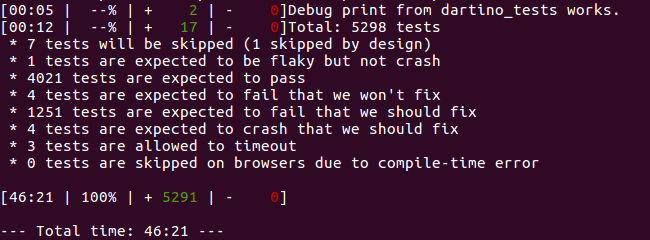
\includegraphics[width=0.7\textwidth]{testovi-mips.png}
  \caption{Резултати тестирања на платформи МИПС.}
  \label{fig:mips}
\end{figure}

\begin{figure}[!ht]
  \centering
  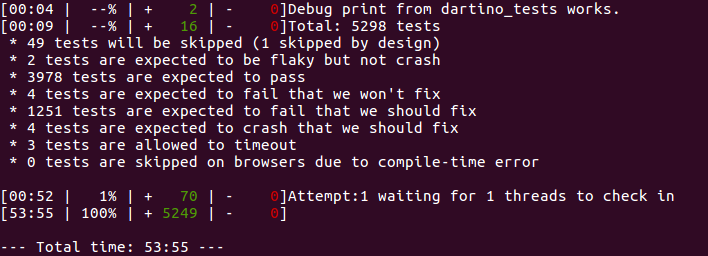
\includegraphics[width=0.7\textwidth]{testovi-arm.png}
  \caption{Резултати тестирања на платформи АРМ.}
  \label{fig:arm}
\end{figure}

\begin{figure}[!ht]
  \centering
  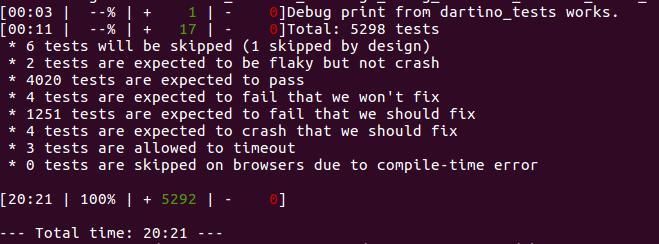
\includegraphics[width=0.7\textwidth]{testovi_x64.png}
  \caption{Резултати тестирања на платформи x86-64.}
  \label{fig:x86}
\end{figure}

\section{Пример апликације у програмском језику Дарт}
\label{sec:aplikacija}


% ------------------------------------------------------------------------------
\chapter{Закључак}


% ------------------------------------------------------------------------------


% ------------------------------------------------------------------------------
% Literatura
% ------------------------------------------------------------------------------
\literatura

% ==============================================================================
% Završni deo teze i prilozi
\backmatter
% ==============================================================================

% ------------------------------------------------------------------------------
% Biografija kandidata

% ------------------------------------------------------------------------------

\end{document} 
